%%%%%%%%%%%%%%%%%%%%%%%%%%%%%%%%%%%%%%%%%%%%%%%%%%%%%%%%%%%%
%
% 2/18일자 "유지현을곁들인.tex"에 추가적으로 작성한 내용임
%
%%%%%%%%%%%%%%%%%%%%%%%%%%%%%%%%%%%%%%%%%%%%%%%%%%%%%%%%%%%%

\documentclass[conference]{IEEEtran}
\IEEEoverridecommandlockouts
% The preceding line is only needed to identify funding in the first footnote. If that is unneeded, please comment it out.

%%%%%%%%%%%%%%%%%%%%%%%%%%%%%%%%%%%%%%%%%%%%%%%%%%%%%%%%%%%%%%%%%%%%%%%%%%%%%%%%%%%%%%%%%%%%%%%%%%%%%%%%%%%%
\usepackage{cite}
\usepackage{amsmath,amssymb,amsfonts}
\usepackage{algorithm}
% \usepackage{algorithmic}
\usepackage[noend]{algpseudocode}

\usepackage{graphicx}
\usepackage{textcomp}
\usepackage{xcolor}
\def\BibTeX{{\rm B\kern-.05em{\sc i\kern-.025em b}\kern-.08em
    T\kern-.1667em\lower.7ex\hbox{E}\kern-.125emX}}
\makeatletter
\newcommand{\linebreakand}{%
  \end{@IEEEauthorhalign}
  \hfill\mbox{}\par
  \mbox{}\hfill\begin{@IEEEauthorhalign}
}
\makeatother

%%%%%%%%%%%%%%%%%%%%%%%%%%%%%%%%%%%%%%%%%%%%%%%%%%%%%%%%%%%%%%%%%%%%%%%%%%%%%%%%%%%%%%%%%%%%%%%%%%%%%%%%%%%%
\begin{document}

\title{Node-RED based Pet Care IoT Solution \\ using MQTT Broker
}

\author{
\IEEEauthorblockN{Haeram Kim}
\IEEEauthorblockA{
\textit{Computer Science and Engineering} \\
\textit{Chungnam National University}\\
Daejeon, Korea \\
haeram.kim1@gmail.com
}
\and
\IEEEauthorblockN{Hyejong Kang}
\IEEEauthorblockA{\textit{Computer Science and Engineering} \\
\textit{Chungnam National University}\\
Daejeon, Korea \\
kanghyejong1001@gmail.com}
\and
\IEEEauthorblockN{Sunghan Kim}
\IEEEauthorblockA{\textit{Computer Science and Engineering} \\
\textit{Chungnam National University}\\
Daejeon, Korea \\
seonghan.kim.cnu@gmail.com}
\linebreakand
\IEEEauthorblockN{Dukho Choi}
\IEEEauthorblockA{\textit{International trade / software convergence} \\
\textit{Chungnam National University}\\
Daejeon, Korea \\
dukho.fin@gmail.com}
\and
\IEEEauthorblockN{Jihyun You}
\IEEEauthorblockA{\textit{Computer and Information Technology} \\
\textit{Purdue University}\\
West Lafayette, IN, USA \\
you62@purdue.edu}

}

\maketitle 

%%%%%%%%%%%%%%%%%%%%%%%%%%%%%%%%%%%%%%%%%%%%%%%%%%%%%%%%%%%%%%%%%%%%%%%%%%%%%%%%%%%%%%%%%%%%%%%%%%%%%%%%%%%%%%%%%%%%%%%%
\begin{abstract}
% `Problem Statment`
While there are an increasing number of households owning pets, it is challenging for owners who leave home often to take good care of their pets.
% `Feature Description`
‘Petification’ is a proposed IoT solution for pet owners to know if their pet is doing well. The functionalities which Petification provides are as follows: Supplying water with Water Supplier device, Feeding the pet with Feed Machine device, Tracking water and food consumption, Tracking water and food remaining amount for each devices, Serving the food by manually or scheduled time, Notifying when water or food is empty, and Displaying visual data with web based dashboard.
% `Methodology`
Load cell and HX711 amplifier is mounted to the both devices to track consumption and remaining amount. MG90S servo motor is mounted to the Feed machine to open and close the food gate and serve certain amount of the food. Raspberry Pi Zero W is mounted to the both devices to control the load cell and servo motor. In a previous study, pet-care IoT solution with a mobile application is already created using Blynk, but Petification uses Node-RED instead of Blynk to connect user with the devices. For controlling message flow, MQTT is used in Petification.
% ----- TESTING & FUTURE PLAN -----
% `Testing`
% To test the Petification, load cell accuracy testing and functionality testing is processed.
% `Testing result`
% The result of testing is that while the accuracy percentage is 99.8\% and Petification can track of consumption and remaining amount, serve food at a right time, notify when water or food is empty, and display visual data to the dashboard, serving amount of food mismatches with desired amount.
% `Future paln`
% Future plan can be enhancing the food gate to serve exact amount of food and adding more devices.

\end{abstract}
\begin{IEEEkeywords}
IoT platform, Node-RED, MQTT, Smart pet care service 
\end{IEEEkeywords}
%%%%%%%%%%%%%%%%%%%%%%%%%%%%%%%%%%%%%%%%%%%%%%%%%%%%%%%%%%%%%%%%%%%%%%%%%%%%%%%%%%%%%%%%%%%%%%%%%%%%%%%%%%%%%%%%%%%%%%%%
\section{Introduction}
% `Project background`
As the number of households living alone increases and the culture of raising pets spreads compared to the past, the number of households raising pets is increasing. This trend is shown in the growth of the pet industry. The growth of the pet industry is one of the indicator of this trend. The profit of the pet industry more than doubles every year over 10 years, from /$48.4 billion in 2010 to /$109.6 billion in 2020 \cite{b1}. Figure 1 shows that households owning a dog consists the largest portion, and the number of families owning dogs has increased from 46.3 million in 2011 to 69 million in 2021.

\begin{figure}[htbp]
\centerline{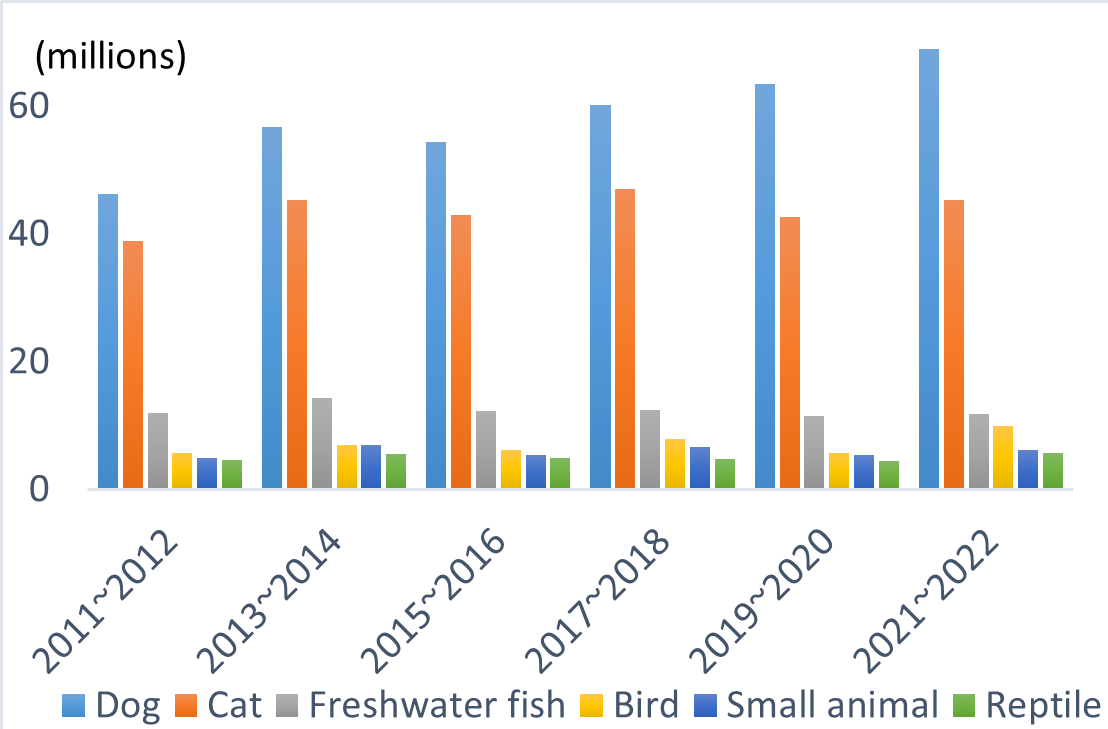
\includegraphics{fig 1.png}}
\caption{Number of U.S. Households That Own a Pet, by Type of Animal
}
\label{fig}
\end{figure}

% `Problem statement 1`
However, along with this trend, demand for tracking pet’s wellness is increased accordingly. One of the demanded service is that tracking pet’s status when the pet is left alone. For those who left home often, it is challenging to take good care of their pets.

% `Problem statement 2`
\indent As a way to solve this problem, Internet of Things (IoT) technology is emerged. A lot of IoT solutions are introduced in the market, and many studies and implementations are suggested. However, most of the suggested IoT solutions uses paid IoT platform, or at least free plan with limited feature. For example, ‘Blynk’ IoT platform is most commonly used \cite{b2} \cite{b3} \cite{b4} \cite{b5}, and ‘Adafruit IO’ \cite{b6} and ‘Freeboard IO’ \cite{b7} are used as well. And while water and food consumption and automatic feeding is commonly supported by previous implementations, there are few solutions that supports device status informations such as device connectivity and remaining amount of food and water. Moreover, error notification is also a less supported feature.

% `Project novelty`
For this reason, The proposed IoT solution provides various notification services for the pets and status of the devices as well as tracking water and food consumption. Furthermore, not to be locked on the limited feature that free plan of commercialized IoT platform provides, the proposed IoT solution is implemented using open-source IoT platform. Thus, the proposed IoT solution uses Node-RED to take advantage of open-source characteristic and many resources.

% `Node-RED`
\\ \indent As a flow-based visual programming tool \cite{b8}, Node-RED makes possible the implementing IoT platform much faster. And also, unlike paid IoT platform, Node-RED is open-source project. By this characteristic, Node-RED supports making user-friendly IoT platform with no feature limitations. Moreover, as a lot of nodes and flows are shared in Node Package Manager (NPM), implementing IoT platform using Node-RED has advantage of utilizing resources.

% `MQTT`
\\ \indent Also, MQTT Protocol is used to manage overall manage flow. Not only the powerful support for MQTT Protocol by Node-RED, but also it is suitable for various IoT solution because of its lightweight characteristic. MQTT is an OASIS standard that provides lightweight message delivery by publish/subscribe model \cite{b9}.

% `Feature Description`
The name of the proposed IoT solution is 'Petification', which includes two key points of system, 'pet' and 'notification'. The definition for pet-care includes overall fields such as providing feed, providing clean drinking water, providing rest areas, exercising regularly, and checking health through veterinarians. \cite{b10}  Among these many pet care fields, Petification is an IoT solution focused on providing feed and water to pets and informing owners of meaningful information. The functionalities which Petification provides are as follows:
\begin{itemize}
\item Supplying water with Water Supplier device.
\item Feeding the pet with Feed Machine device.
\item Tracking water and food consumption.
\item Tracking water and food remaining amount for each devices.
\item Serving the food by manually or scheduled time.
\item Notifying when water or food is empty.
\item Providing the device status.
\item Displaying visual data with web based dashboard.
\end{itemize}

\section{Related Literature}
This chapter will be explained with hardware and platform perspective respectively. In the hardware part, used devices are compared with them of Petification, and used IoT platform and provided feature will be compared with present research in the platform part.

\subsection{Hardware}
In the previous study conducted by P. N. Vrishanka \textit{et al.} \cite{b11}, automated pet feeder is proposed. To implement it, ultrasonic distance sensor and SG90 servo motor were mounted to Arduino Uno R3. An ultrasonic distance sensor is used to determine the remaining food amount by measuring the distance from the entrance of the feed container to the inside of the bowl.

However, the feed machine of Petification used load cell sensors to determine the remaining food amount, as it is difficult to use ultrasonic waves to measure the amount of feed accurately.

In the previous study conducted by Rogerio Nogueira \textit{et al}, \cite{b12} , Rotary Valve and DC motor were used to provide feed. And in the previous study conducted by Vania \textit{et al}, \cite{b13}, propeller blade and DC motor were used.

However, the problem with using a rotary valve or propeller blade is that the feed can’t be provided with the exact weight. This is because the amount of feed to be provided to the pet is determined based on the serving unit contained in one space. Thus, when the feed machine tries to provide a certain weight of feed with the rotary valve or propeller blade, there is always the possibility of providing more than the intended weight, even if the error for load cell is not concerned. The Petification feed machine does not use a rotary valve but uses a gate that can block the feeder container outlet because it has the advantage of being able to adjust the amount of feed to be supplied in more detail than the rotary valve method.

In addition, both \cite{b12} and \cite{b13} uses a DC motor to provide feed through continuous rotation of the rotary valve. However, the feed machine of Petification uses a servo motor because they need more precise control than free continuous rotation.\cite{b14} 

\subsection{Platform}
  The previous study conducted by Y. Chen \textit{et al.} \cite{b5}
proposed a pet care IoT system that provides food and water consumption, number of defecation, and defecation duration. It was developed through Arduino IDE and provides features above with numbers and visual statistics in real-time using “Blynk” as an IoT platform.

The previous study conducted by T. Sangvanloy \textit{et al.} \cite{b4} 
proposed a pet care IoT solution that visualizes the daily food consumption in real-time and automatically feeds the pet according to the scheduled time. It was also implemented using “Blynk” as an IoT platform.

But, non of the two studies above provide information on device status. Although tracking water and feed consumption is an important feature in pet care IoT solutions, keeping track of IoT devices’ status is also an important feature. Petification provides the status of feed machines and water supply machines, such as device connectivity, error existence, and the amount of feed or water remaining in the device. Moreover, Petification provides an error notification feature that notifies users when the error occurred, such as when water or feed is empty.

From the used platform perspective, the above two studies commonly used ‘Blynk’ as an IoT platform. However, Petification uses Node-RED instead of ‘Blynk’ to take advantage of visual programming, openly pre-developed flows and nodes, and various notification means.

\section{Methodology}
\subsection{Overview}
As MQTT is the main messaging protocol for petification and MQTT uses TCP/ IP protocol stack, each devices are connected to the Access Point (AP) through Wi-Fi. Thus, all the messages published from devices are sent to the AP with Wi-Fi, and then they are sent to the Petification platform through internet. Petification platform processes the messages and send the processed data to the users in form of web dashboard page, E-Mail, and WhatsApp message. On the contrary, user can send requests with the web dashboard to the platform. While some requests require only the platform, the requests to activate the actuator are forwarded to the device with the help of the platform. In summary, user and devices communicates bidirectionally through the platform. The overview for Petification is shown in figure 2.

% `Overview.png`
\begin{figure}[htbp]
\centerline{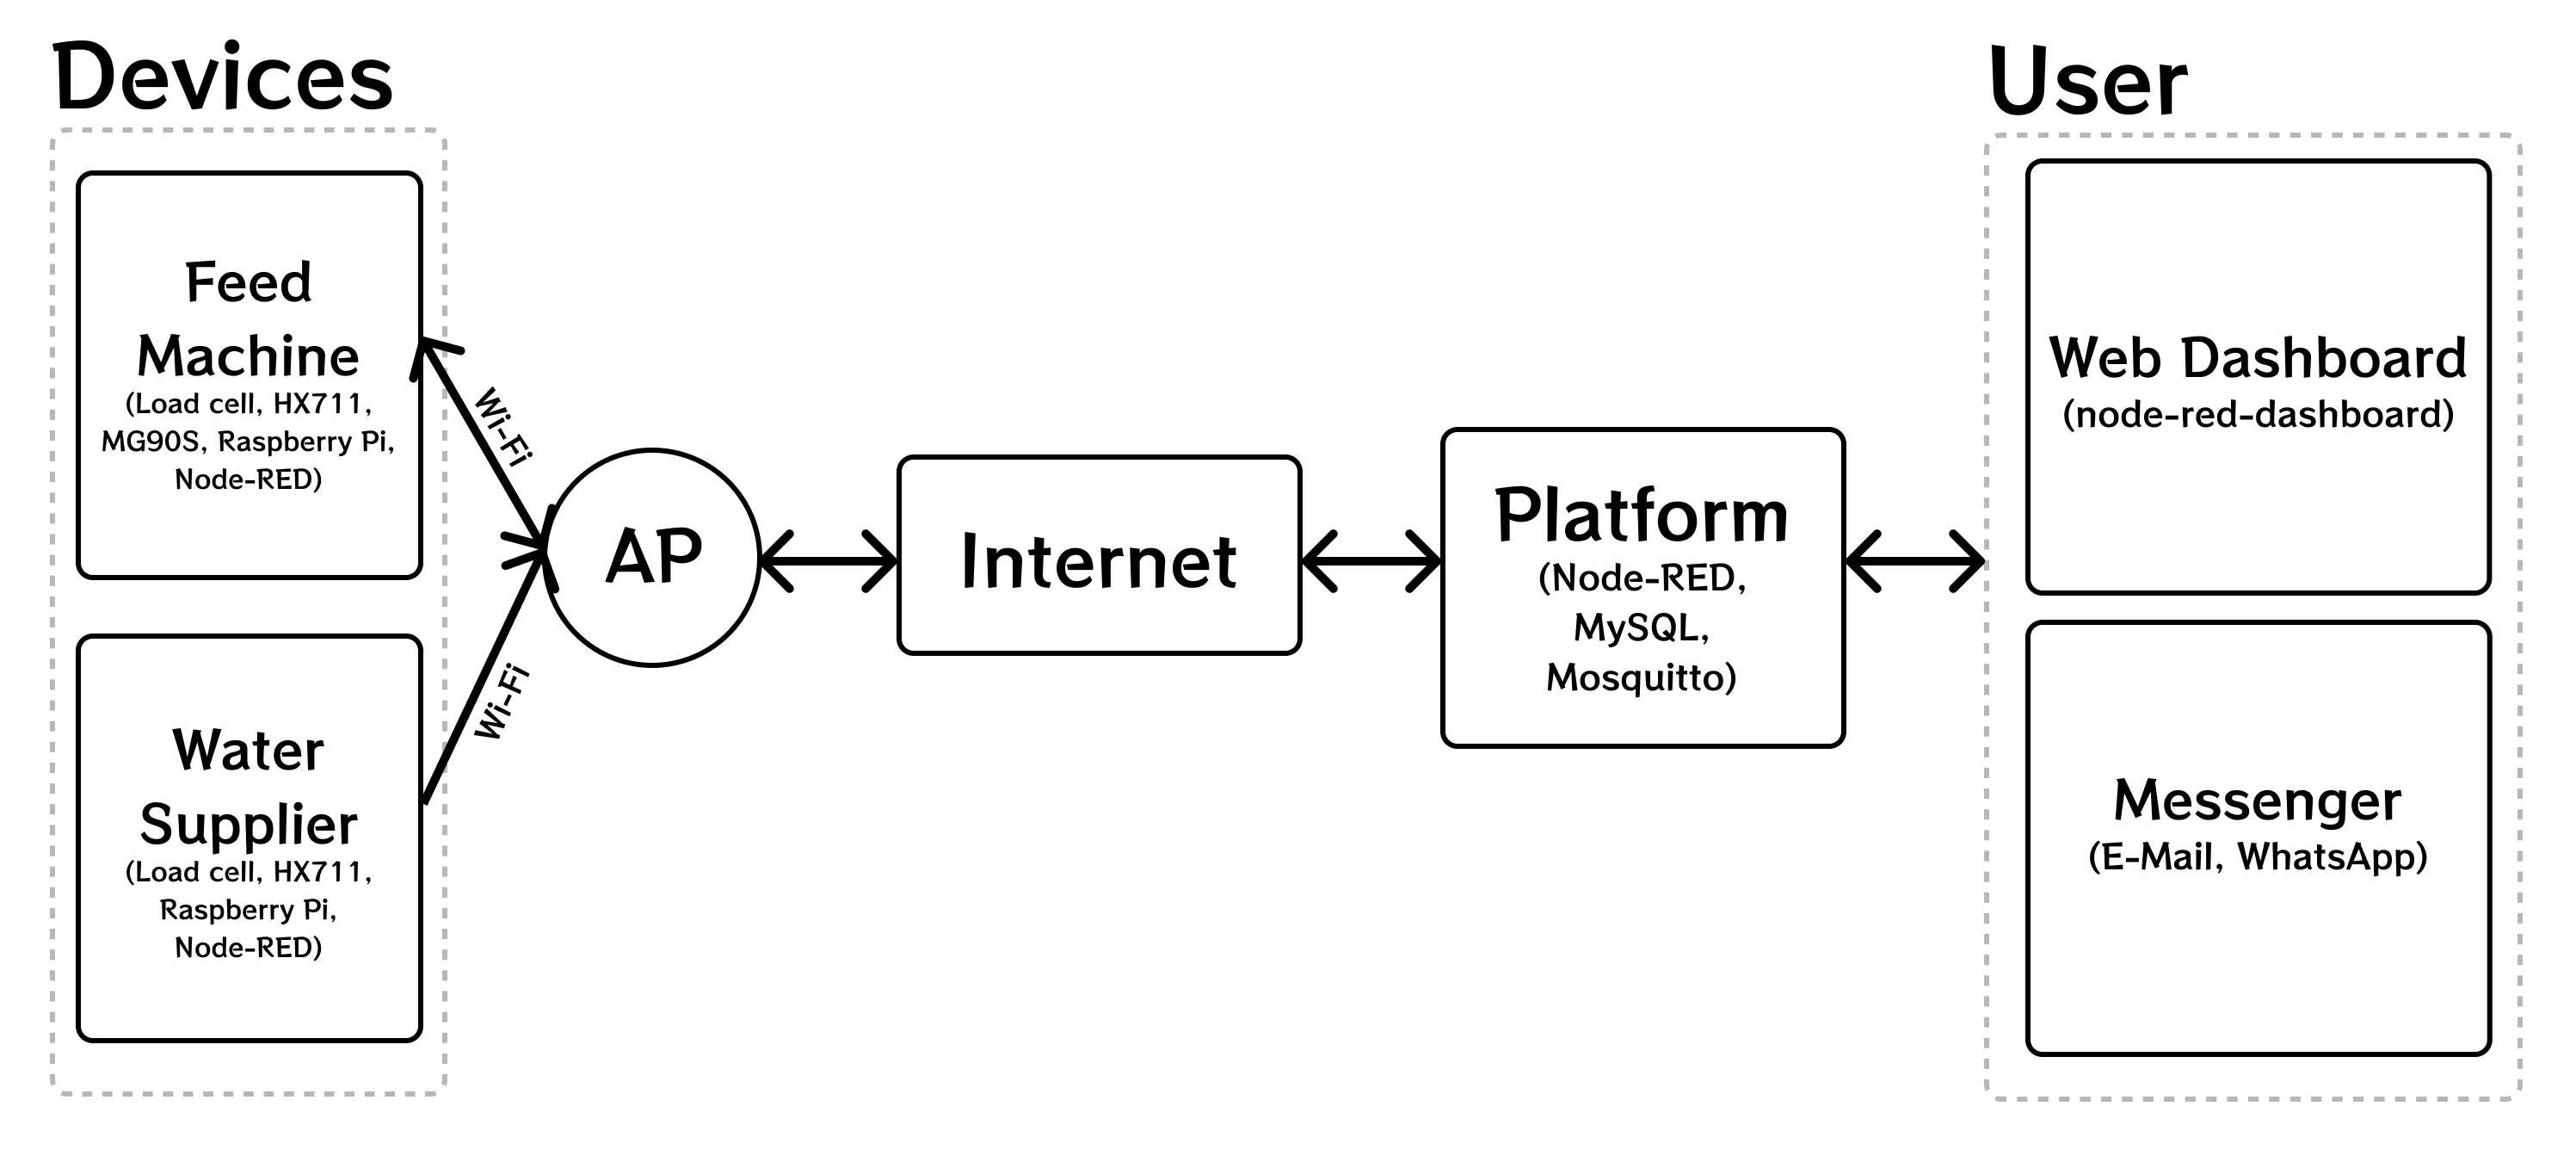
\includegraphics[width=0.5\textwidth]{Overview.png}}
\caption{Petification overview.}
\label{fig}
\end{figure}

\subsection{Used Technology}
\subsubsection{Hardware}
The load cell sensor serves to convert the weight or force acting into an electrical analog signal \cite{b15}. In the present research, three load cells which weighs up to 5kg with 1g accuracy are used.

All the load cells are mounted to the microcontroller through load cell amplifier. In Petification, three HX711 module is used as load cell amplifier. HX711 converts an analog signal into a digital signal, amplifies a measured value of a low load cell, and then transmits the value to another microcontroller \cite{b16}. 

The servo motor is a rotary or linear actuator that rotates and pushes a machine \cite{b17} and one MG90S servo motor is used.

The role of the microcontroller is orchestrating all the sensors and actuators and communicating with IoT platform. For microcontroller, two Raspberry Pi Zero W are used.

\subsubsection{Node-RED}
Node-RED is a flow-based visual development tool that is easy for developers and non-developers to develop programs. Node-RED is popularly used to connect hardware devices, APIs, and online services \cite{b18}.
% `Strengths of the Node-RED`
One of the Node-RED’s operational strengths is that it can run on various environments such as local, Raspberry Pi, Docker, Cloud Instance, and \textit{et al}. \\
% `Core nodes we use`
% `1. Network Node - MQTT, HTTP`
% `2. Exec Node`
\indent In Node-RED core package, a lot of nodes are pre-installed by default. ‘HTTP node’ and ‘MQTT node’ is provided to help configuring network. Also, Node-RED core package provides ’Exec node’ which helps executing system command. Being able to execute system command means that other programming languages can be integrated to the flow. For example, python code file can be executed with the help of ‘Exec node’. \\
\indent Node-red is open-source project and not only Node-RED itself but also various nodes are being distributed through Node Package Manager (NPM). Thus, users can share their nodes or flows, and a lot of contributed nodes are available in NPM.
% `Supported nodes that we use`
% `1. Dashboard - node-red-dashboard`
% `2. Database - MySQL`
% `3. Social - EMail, WhatsApp`
User interface (UI) can be configured using Node-RED’s ’node-red-dashboard’ package. It also supports appending Cascade Style Sheet (CSS) and JavaScript code to the dashboard, so user-friendly UI is easily configured \cite{b19}. Furthermore, Node-RED has the advantage of allowing users to easily access the database and manipulate data. There are various nodes to access database, such as ‘node-red-node-mysql’ which helps accessing to the MySQL server. Also, a lot of nodes are distributed to send notifications to users, such as ‘node-red-node-email’ that helps sending e-mail, and ‘node-red-contrib-whatsapp-cmb’ that helps sending WhatsApp message. \\
% `Node-RED and IBM`
\indent Node-RED is made by International Business Machines Corporation (IBM), and IBM plans to increase its contributor base as an open-source for the sustainability of Node-RED. \cite{b20}.

\subsubsection{MQTT}
MQTT stands for Message Queuing Telemetry Transport and is the oldest Machine to Machine (M2M) protocol for IoT. It is an ISO standard Publishing-Subscribing-based messaging protocol designed for lightweight M2M communication in a limited network. All MQTT messages have their own topics, and MQTT clients can send and receive data by posting messages to MQTT  or subscribing to topics for those messages. TCP is used as a transport protocol, and TLS/SSL can be used for security. This means connection-oriented between Client-Brokers. In the MQTT protocol, three levels of quality of service (QoS) are used: QoS0(), QoS1(), and QoS2(). The MQTT protocol has a small message size and message overhead. In addition, due to low power consumption and resource consumption, it is evaluated as a suitable protocol for use in the IoT field.
\cite{b21}

\paragraph{MQTT vs Other Protocols(CoAP, AMQP, HTTP)}
\hfill \break
Protocols to consider in an IoT platform aside from MQTT that was mentioned earlier include
CoAP, AMQP, and HTTP.They could be categorized by CoAP which uses UDP as the transport protocol, and MQTT, AMQP, and HTTP that uses TCP. From this project’s perspective, CoAP uses UDP as the transport protocol. The size of the message and the overhead is small which is an advantage, however, as the UDP’s characteristic the packet delivery is not guaranteed. Furthermore, CoAP is specialized to devices that support UDP and UDP analog so it is not suitable to support all devices. Next, AMQP uses TCP as the transport protocol. Compared to MQTT, reliability, security, provisioning, and interoperability is higher. However, because of that the message size and the overhead is a lot bigger compared to MQTT and the power and resource consumed by the device are large. Finally, HTTP is a protocol for the web, thus it could result in delays between the device and the platform’s data flow. Additionally, the power and resource consumed by the device are similar to AMQP which is a downfall.

Therefore, MQTT utilized TCP as the transport protocol to guarantee the packet delivery and has an appropriate amount of message size and overhead. Furthermore, the consumption of power and resource is minor which is an advantage since the time of using the device is important.
This concluded that the MQTT protocol is suitable for the IoT platform project composing the
message broker. The message broker uses Mosquitto which is the MQTT protocol implemented.\cite{b21} 

\subsubsection{Mosquitto}
Mosquito is an open-source message broker implementing MQTT protocol versions 5.0, 3.1.1, and 3.1 and is provided by Eclipse. It is also lightweight and suitable for use in all devices, from low-power single-board computers to full servers.\cite{b22}

Several programs are implementing MQTT, such as EMQ, HiveMQ, Mosquito, and VerneMQ. A study comparing each of the programs suggested that in situations where availability is not significant, using Single Broker and Persistence Setting is a simpler way to configure Message Broker than using clustered Broker \cite{b23}. In addition, in the context of using Persistence Setting in Single Broker, Mosquitto had close to 0 percent probability of message loss and message order mixing, and the probability of receiving duplicate messages was significantly lower than other programs \cite{b23}. Thus, this research uses Mosquitto with persistency setting as a single message broker.

\subsubsection{MySQL}
MySQL is a fast, flexible, and easy-to-use database with RDBMS (relational database management system). The combination of MySQL's secure processing and reliable software provides effective transactions for large projects, so it is flexible with open sources. MySQL is also excellent in terms of data security because it is evaluated as having the safest and most reliable database management system \cite{b24}. In addition, MySQL is considered a suitable database to manage effective data flows because it has good compatibility with Node-RED \cite{b24}.

\section{Hardware Design}

\subsection{Feed Machine}
Feed Machine is one of the device attached to proposed platform. The Feed Machine has 2 main functionalities: Serving food to the pet and Reporting weight of the food bowl and container to the platform. To serve food to the pet, servo motor is mounted to open and close the food gate. As in Figure 3, the servo motor gives food in an open/close type. Food serving is done with the help of gravity; After food gate is opened, food rolls down the slope, and thus food is served. By closing the food gate Feed Machine stops serving of the food. To measure the weight of the food bowl and container, two load cell is mounted under the each of them. Like in Figure 4, each load cells are connected with HX711 Amplifier to convert analog signal to the digital signal. Also, as in Figure 5., Load cell sensors are installed between wooden boards to measure the weight. Additionally, in Figure 5, a food container carries food through a slide into a food bowl. All the sensors and a servo motor is attached to Raspberry Pi Zero W.

\begin{figure}[htbp]
\centerline{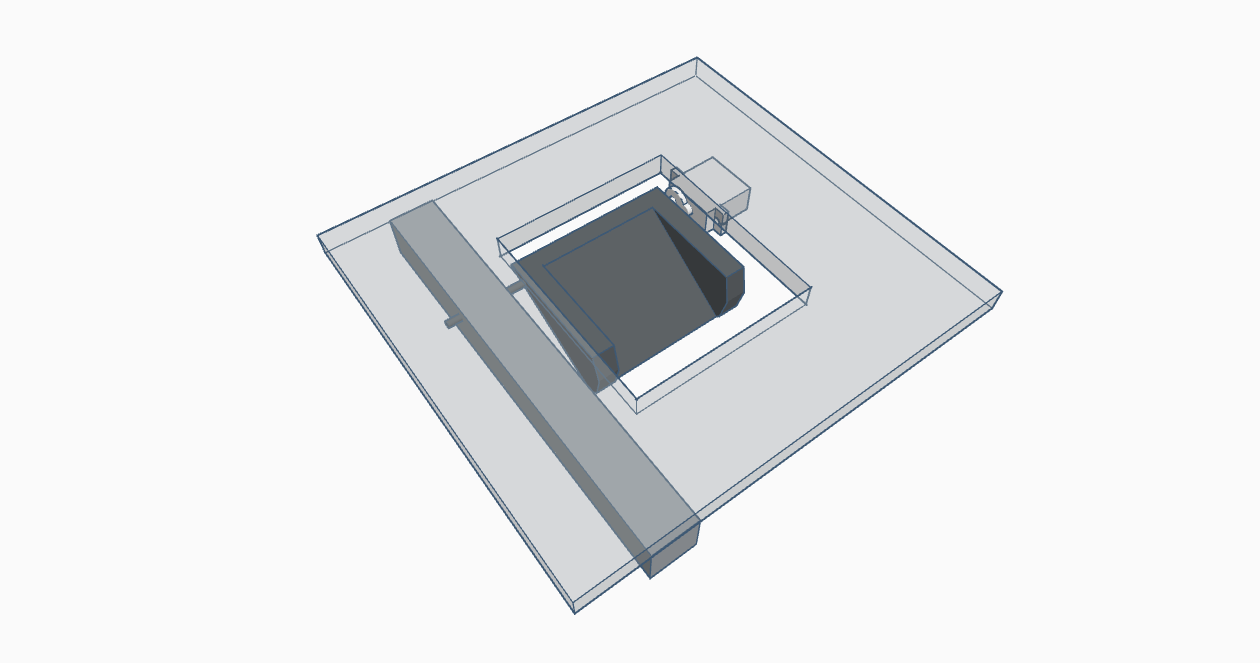
\includegraphics[width=0.5\textwidth]{servo_gate.png}}
\caption{Block diagram for Feed machine and Water supplier.}
\label{fig}
\end{figure}

\subsection{Water Supplier}
Water supplier is also a device attached to the proposed platform.
The water supplier has a functionality that reporting total weight of the water in water supplier.
Similar to a feed machine, to measure the weight of water in water supplier a load cell is mounted under water supplier. In addition, like in Figure 4.,the HX711 amplifier is used to convert analog signals into digital signals. As in Figure 5., like a feed machine load cell sensors are installed between wooden boards to measure the weight. Both types of sensor and RaspberryPi are same with feed machine. 

\begin{figure}[htbp]
\centerline{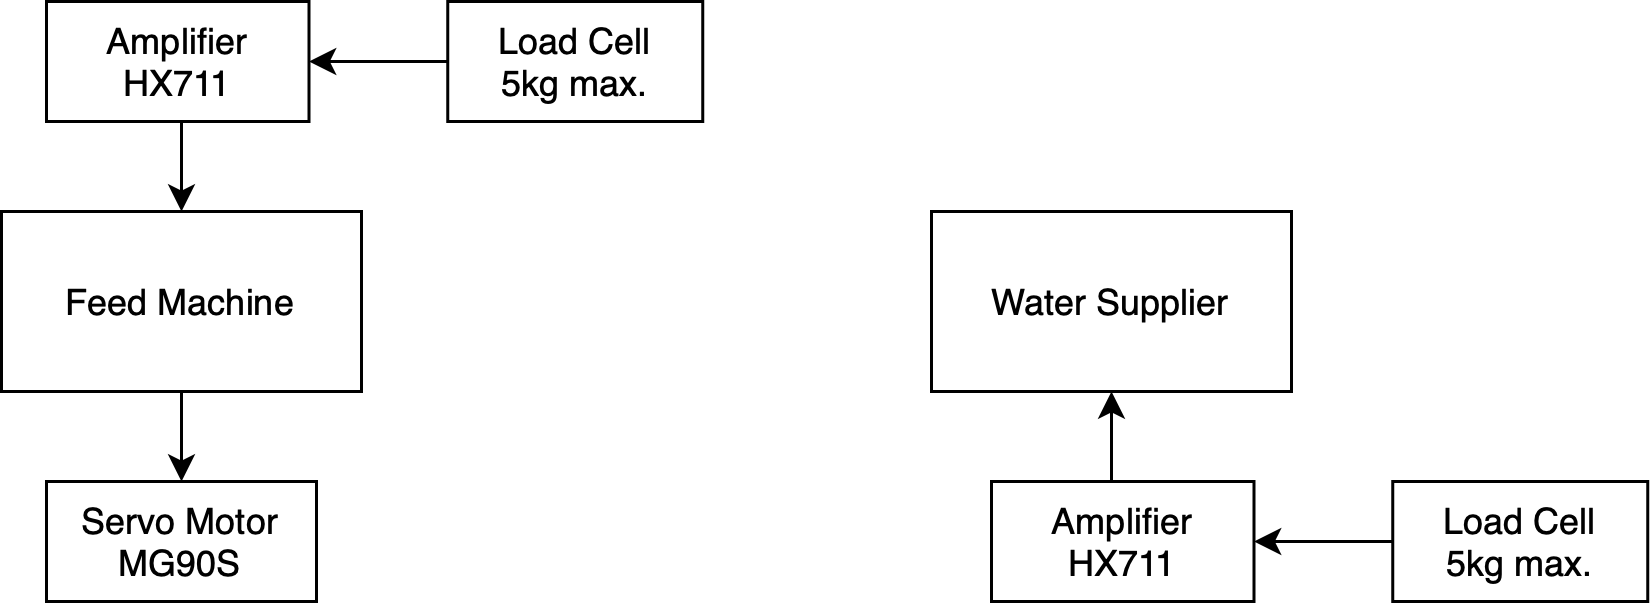
\includegraphics[width=0.5\textwidth]{hardwareBlock.png}}
\caption{Block diagram for Feed machine and Water supplier.}
\label{fig}
\end{figure}

\begin{figure}[htbp]
\centerline{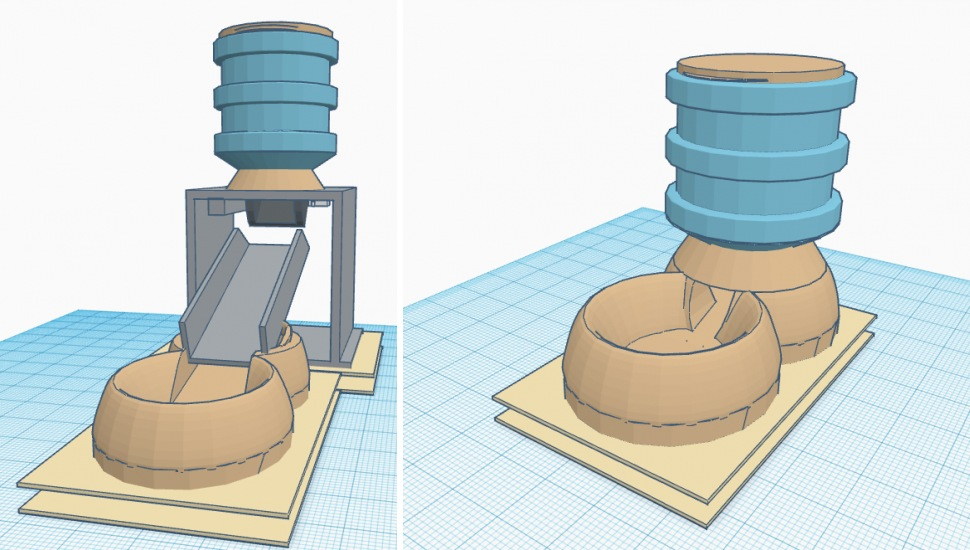
\includegraphics[width=0.5\textwidth]{Feed Machine & Water Supplier.jpg}}
\caption{Feed Machine and Water Supplier CAD Image}
\label{fig}
\end{figure}



\subsection{Activity Diagram for Hardware Design}

% `deviceSetup.png`
\begin{figure}[htbp]
\centerline{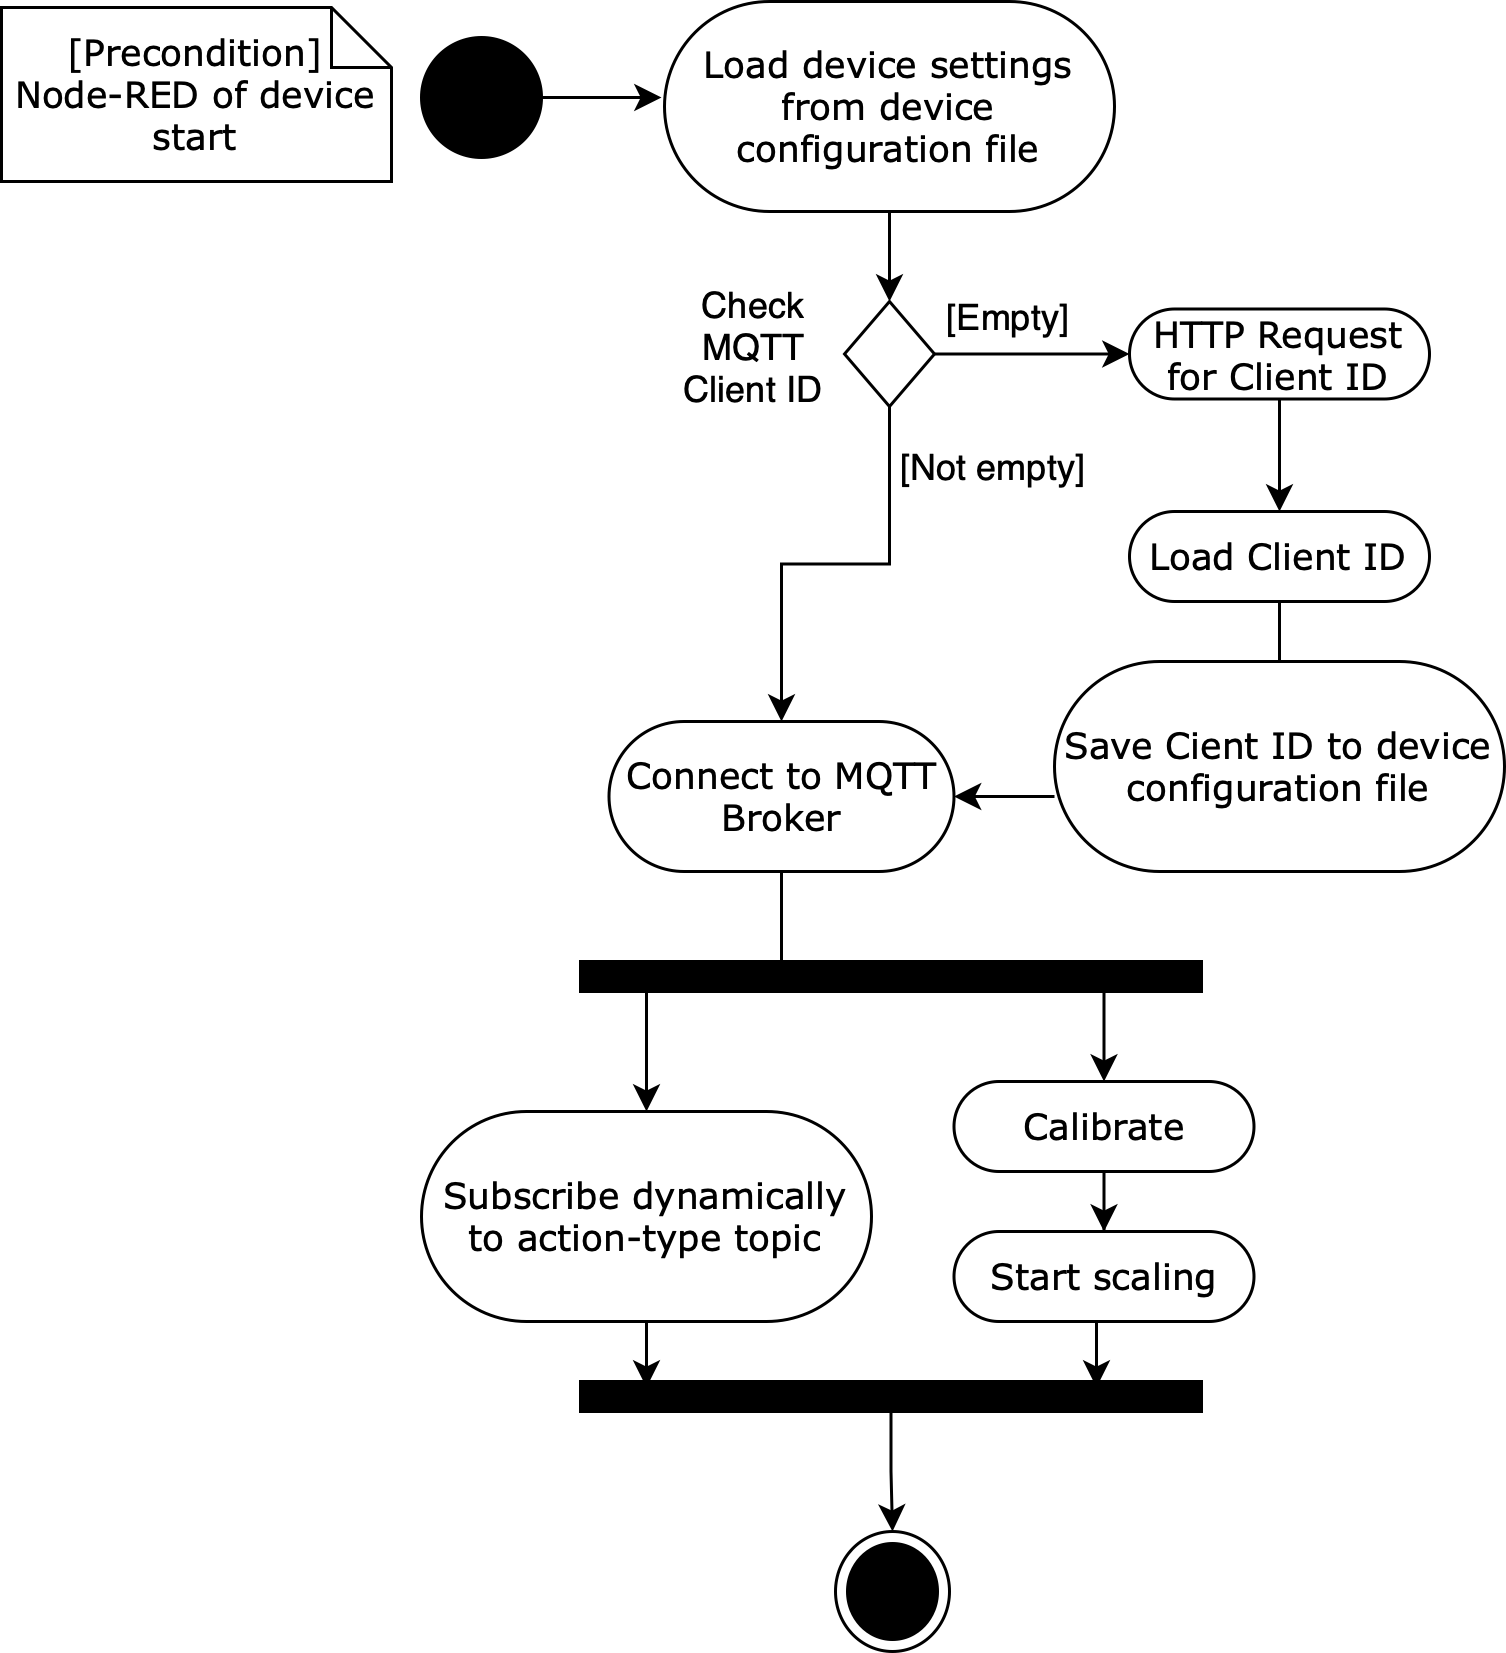
\includegraphics[width=0.5\textwidth]{deviceSetup.png}}
\caption{Activity Diagram for Device Setup.}
\label{fig}
\end{figure}

\paragraph{Device Setup}
In Figure 6 when Node-RED is initially executed in the device, the device settings file is loaded from the configure files.
Thereafter, check the MQTT Client ID to connect directly to the MQTT broker if the MQTT Cid exists, and if the Cid does not exist, the Cid is issued through HTTP Request, stored in the setup file, and connected to the MQTT broker. When connected to an MQTT broker, Device commonly starts scale weight after calibration, and at the same time subscribes to the action type topic to listen to action messages coming from outside.

\paragraph{Calibration}
Petification uses load cell weight function to measure the weight of the pet’s food and water,
calibration takes place to measure the weight with load cells.
In the process of calibration, we need to choose an object to be used as the standard weight. In
this project, we set a 500ml bottle of water as 500 g.
Using the selected object (500ml bottle of water in this case), the load cell was used to measure
the force the object applies to the load cell due to its weight.
The bottle of water has been measured several times and the average of the data is calculated.
Then the reference unit can be calculated by dividing the calculated average by the weight of the
object.
Depending on the load cell and the reference unit, there is a possible error.
The reference unit is used as the factor of set\_reference\_unit() which is the method of hx711 to
calculate the measurement and calculates the measurement depending on the standard weight to
be ready for wight measurement. Using this, it is possible to measure the desired weight, and the
weight could be calculated through the measured force measured by the load cell.

% `publishScaleError.png`
\begin{figure}[htbp]
\centerline{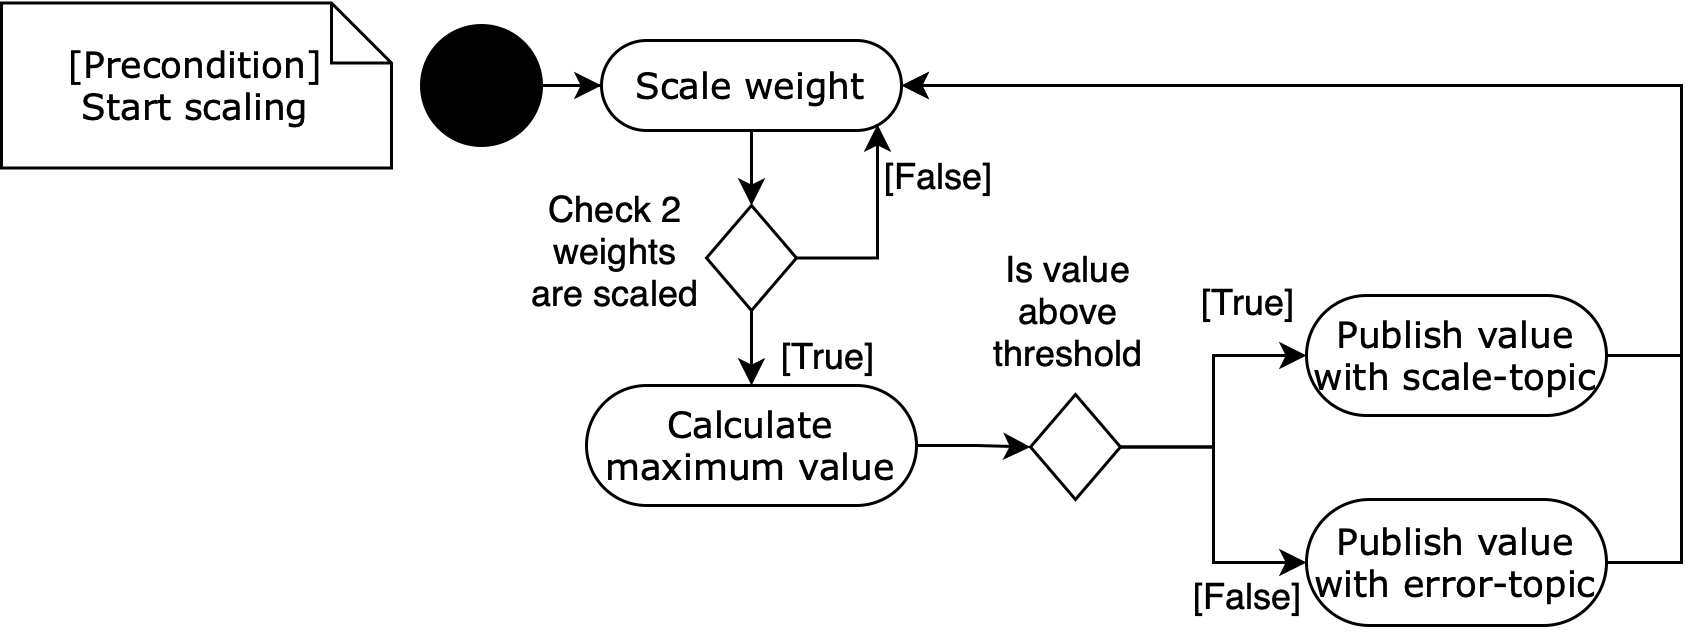
\includegraphics[width=0.5\textwidth]{publishScaleError.png}}
\caption{Activity Diagram for Publishing Scale and Error Detection}
\label{fig}
\end{figure}

\paragraph{Publishing Scale and Error Detection}
In Figure 7, when weight data begins to be collected after scaling in Device, two weight values are collected. If two do not gather, repeat the scale process to collect two values and process them at once. Afterwards, a large value is selected from the two scaled data, and if the scale value is large compared to the threshold, the scaled weight is published, and if not, an error-topic message is published.

% `actionMessageReceived.png`
\begin{figure}[htbp!]
\centerline{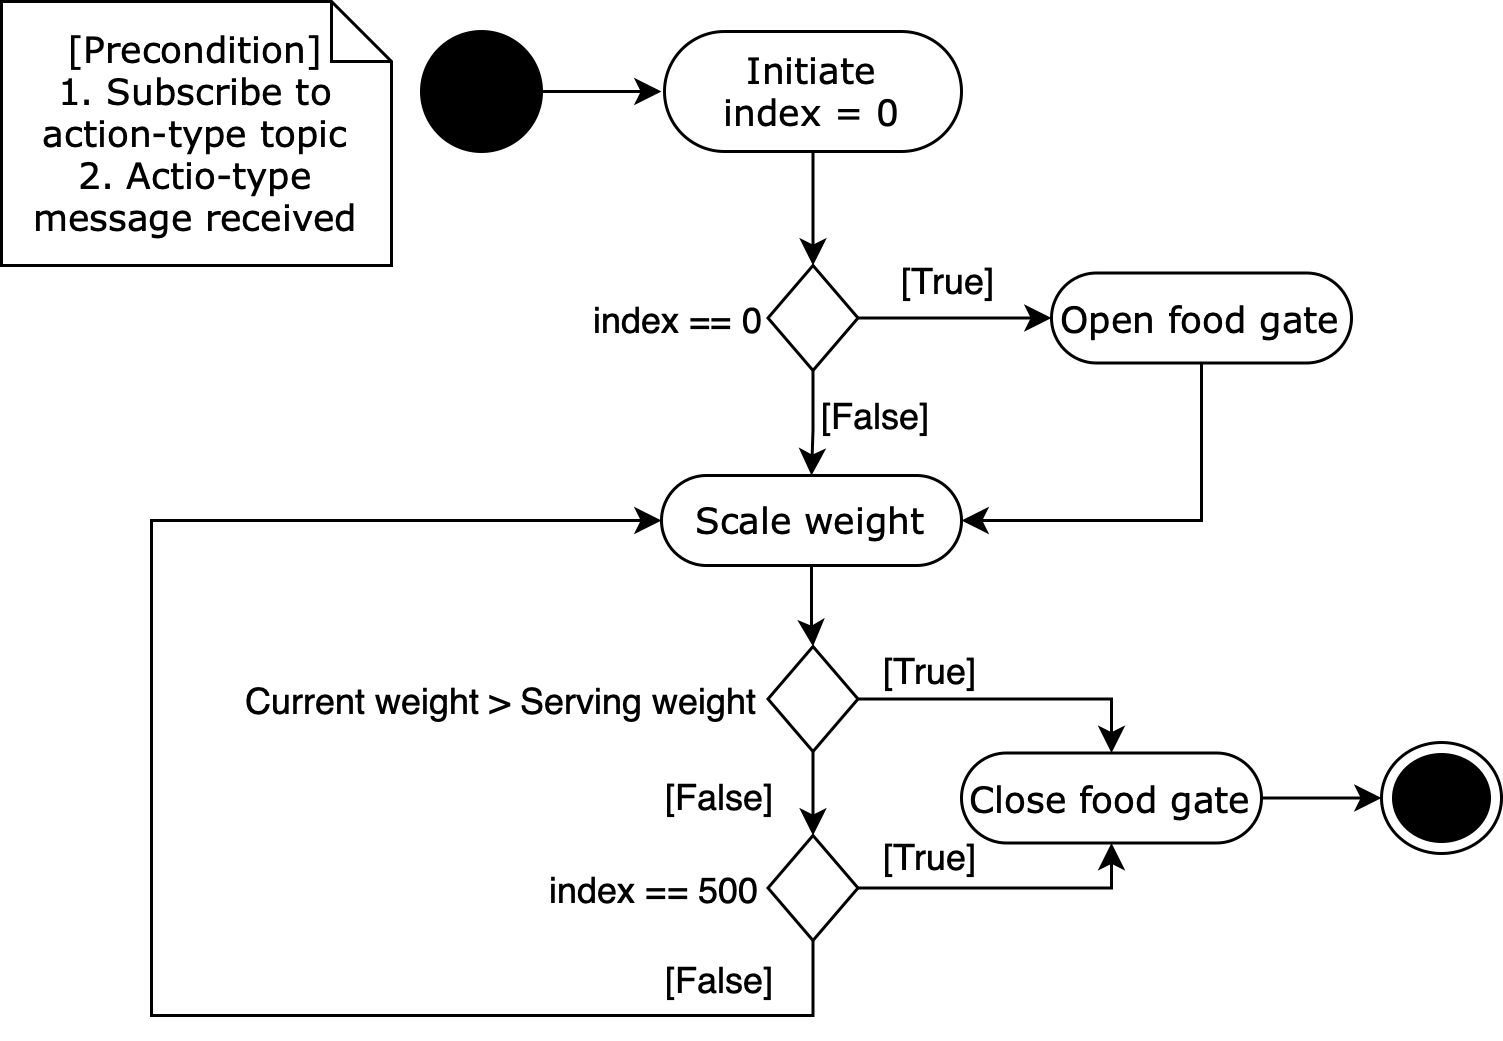
\includegraphics[width=0.5\textwidth]{actionMessageReceived.png}}
\caption{Activity Diagram for Automatic Feeding.}
\label{fig} 
\end{figure}

\paragraph{Automatic Feeding}
In Figure 8, device subscribes to MQTT messages for Action-type topics.
Accordingly, Device can receive an Action-type message, and if it receives a message, it initializes the index to 0 using a loop statement, opens the food gate, and feeds.
Weight scaling continues and repeats while the current weight is less than the weight input by the user.
If the current weight is greater than the user input value, close the food gate.
The max itertaion count is 500, and during that loop, the current weight is less than the input weight, and the food gate is automatically closed when the iteration ends.

\section{Software Design}
% `NEED TO ADD INITIAL paragraph`
\subsection{Blocks}
The platform for petification consists of 9 blocks: MQTT Message Broker and Database are running on independent processes, while MQTT Manager, Time-series Manager, Rule Engine, Device Manager, User Manager, Schedule Engine, and UI Dashboard Manager are running on Node-RED. Figure 9
% `Blocks.png`
shows the block diagram of Petification and interaction between devices and platform blocks.

% `Blocks.png`
\begin{figure}[htbp]
\centerline{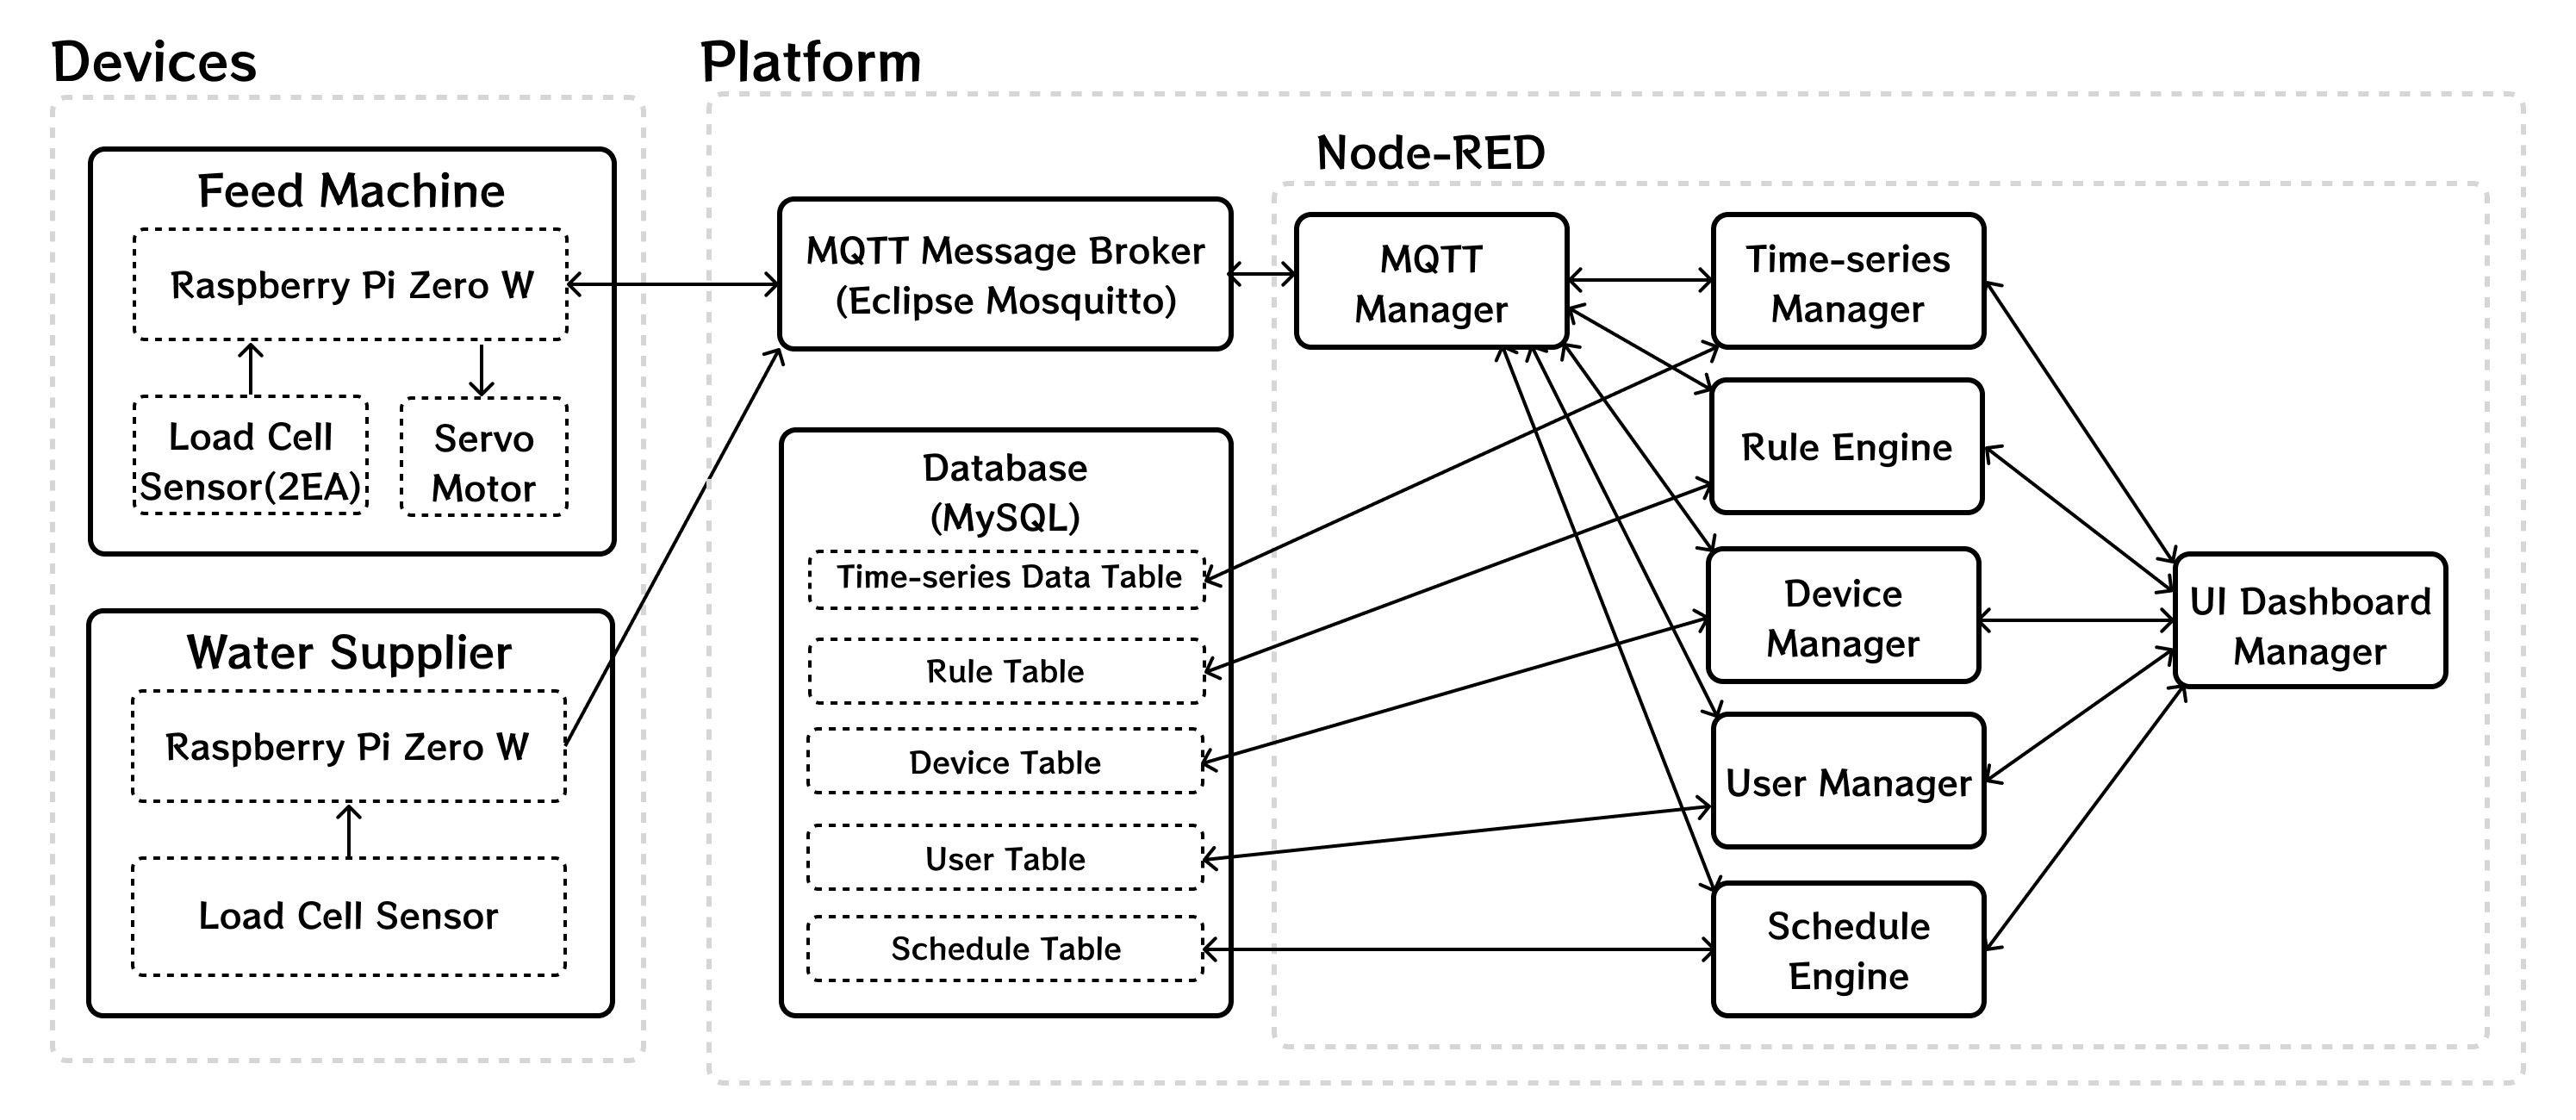
\includegraphics[width=0.5\textwidth]{Blocks.png}}
\caption{Platform block diagram and interaction between devices.}
\label{fig}
\end{figure}

\subsubsection{MQTT Message Broker}
\hfill \break Petification uses MQTT Protocol to control the message flow. Thus, Mosquitto v1.4.15 was installed and running on the platform server to act as an MQTT Message Broker. Feed machine, water supply machine, and Node-RED are connected to the MQTT Message Broker as a client, and MQTT Message Broker mediates Node-RED to Device communication and reverse-way communication (Device to Node-RED).

\subsubsection{Database}
\hfill \break To store data efficiently and safely, a Database block is included in the platform. As a Database block, MySQL v5.7.37 is installed and running on the platform server. The database stores various data, such as all the MQTT messages (in a Time-series Data Table), message-based action execution rules (in a Rule Table), information for the connected devices (in a Device Table), user information (in a User Table), and time-based action execution rules (in a Schedule Table).

\subsubsection{MQTT Manager}
\hfill \break MQTT Manager in the Node-RED is the gateway for MQTT messages to enter Node-RED. The main purpose of this block is to convert incoming MQTT messages to give convenience to other Node-RED-based blocks. To achieve it, this block receives all the messages by subscribing to all the MQTT message topics. And then it parses message topic and payload to provide useful information such as the MQTT username and client id. These pieces of information are used in other Node-RED-based nodes in further progress.

\subsubsection{Time-series Manager}
\hfill \break Managing Time-series Data Table of Database is the main purpose for Time-series Manager block. This block provides 3 types of ReST APIs for managing time-series data: Inquiring record feature (with HTTP GET method), Changing record validity (with HTTP PATCH method) and Deleting record (with HTTP DELETE method). 

\subsubsection{Rule Engine}
\hfill \break The purpose of Rule Engine is to activate actions according to MQTT messages. It cooperates with the Rule Table of Database to activate the action. Designing logic of the Rule Engine is inspired by the book, “Build Your Own IoT Platform” \cite{b25}. For every published message, Rule Engine searches for all rules where the rule's message pattern satisfies the message content. Actions that corresponded to the rules are defined as ReST API form, thus activating action will be progressed as sending an HTTP request. It also provides ReST APIs for adding, modifying, and deleting rules. Some ReST APIs for actions are defined in another block, whereas some APIs are defined in Rule Engine, such as sending notifications.

\subsubsection{Device Manager}
\hfill \break Handling devices that are attached to the platform by users is the main purpose of the Device Manager block. It provides ReST APIs that can add a new device to the platform (with HTTP POST method), modify the status of the device (with HTTP PATCH method), delete a device (with HTTP DELETE method). And it also provides functionality for publishing action-type message to the specific device.

\subsubsection{User Manager}
\hfill \break The purpose of the User Manager block is to provide interface for modifying user settings. Users can manage these 4 settings: Notification, Email address, WhatsApp information, and timezone where the user lives.  In order to support global users, Timezone settings is included. As all the times that platform uses and database stores uses Coordinated Universal Time (UTC) timezone, converting time of the user to the UTC is necessary. This setting is especially important when user adds new schedule by using Schedule Engine, and when providing local time to the user in the Dashboard.
% token이랑 uname을 여기서 말해야될거같기도 하고

\subsubsection{Schedule Engine}
\hfill \break Handling and executing schedule is the main functionality for this block. For schedule execution, it cooperates with the Schedule Table in the Database. Every minute, the Schedule Engine checks the Schedule Table and executes the actions that are scheduled to be activated at that time. Also, this block provides ReST APIs that can create, read, update and delete the schedule.

\subsubsection{UI Dashboard Manager}
\hfill \break Dashboard Manager is to provide Graphical User Interface (GUI) to the user. By using this block, users can be provided the status of water and food remaining and consumption visually. It also provides buttons to serve food and input areas to set user settings.

\subsection{Activity Diagram for Software Design}
\subsubsection{Receiving Scale Message}
\begin{figure}[htbp]
\centerline{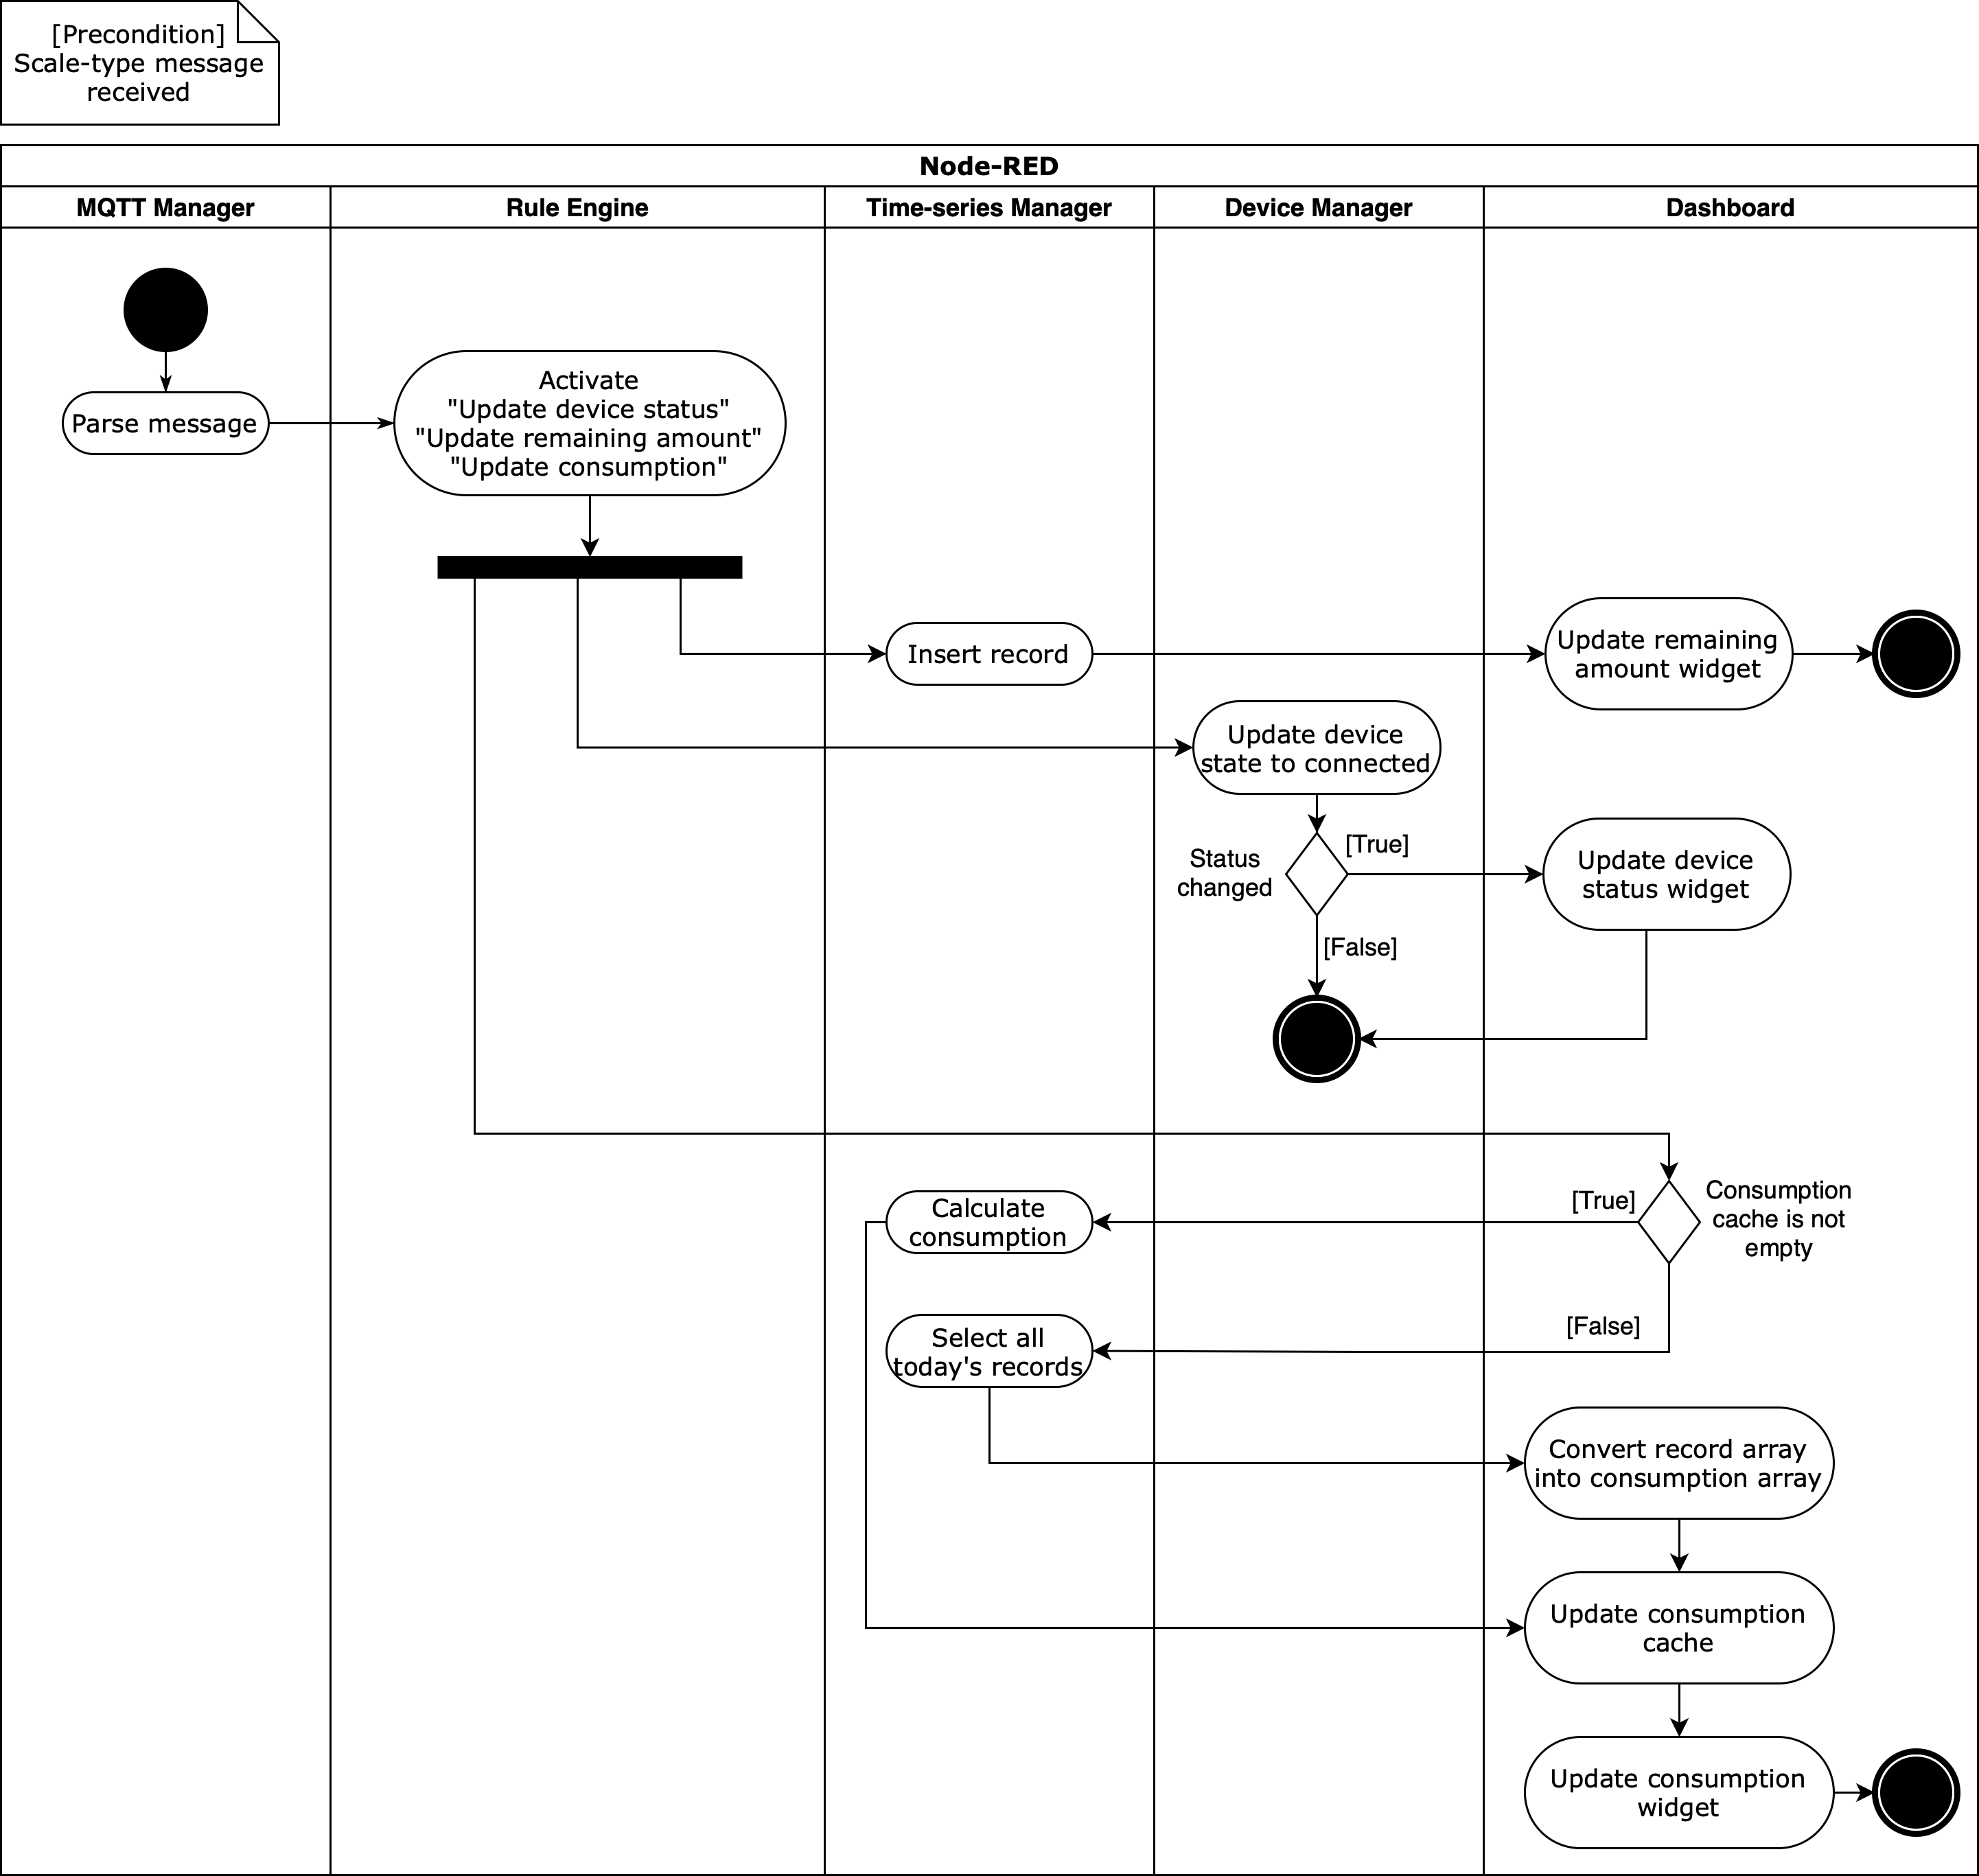
\includegraphics[width=0.5\textwidth]{scaleMessageReceived.png}}
\caption{Activity Diagram for Receiving scale message.}
\label{fig}
\end{figure}

Activity Diagram for Receiving scale message is shown in figure ?
% `scaleMessageReceived.png`
. When a scale-type message is received to the platform, MQTT Manager parses the message and toss it to the Rule Engine. After that, Rule Engine activates 3 rules and these rules proceeds in parallel: Update device status, Update remaining amount, and Update consumption. In activating Update device status, Device Manager block updates the device’s status and toss the changed status to the Dashboard block only if status of the device is changed. For Updating remaining amount, the scale-type message is stored the to Time-series Data table by Time-series Manager block. After storing the message, payload of the message is tossed to the Dashboard block to update remaining amount widget.
Lastly, for updating consumption, platform checks the consumption cache firstly. When consumption cache is empty, consumption array is loaded to the cache, and when it’s not, consumption is calculated and appended to the consumption array of the cache. To load cache, Dashboard request all the records that are stored after the midnight of the day for the topic of received message. Consumption array is prepared by calculating all of the consumptions for that records. After consumption cache is updated, Dashboard block updates the consumption widget based on the prepared consumption cache.
The basic idea for calculating consumption is comparing current and previous scale. When pet consumes food or water, scale for that will be decreased. Thus, consumption can be derived by accumulating each decrease amount. The pseudo code for calculating consumption is shown in algorithm 1. Initial value for decrease amount is set to 0, and decrease amount is updated to difference between previous and current scale only when the previous scale is bigger than the current scale. By adding decrease amount to the previous consumption, current consumption can be derived.

\begin{algorithm}
\caption{Calculate consumption}\label{algo}
\begin{algorithmic}[1]
    \Procedure{CalcConsumption}{}
        \State $prevConsumption \gets \text{previous } \textit{consumption}$
        \State $currScale \gets \textit{scale} \text{ of received message}$
        \State $prevScale \gets \textit{scale} \text{ of  previous record}$
        \State $decrease \gets 0$
        \If{$precScale \neq \textit{null} \And prevScale > currScale$}
            \State $decrease \gets prevScale - currScale$
        \EndIf
        \Return $prevConsumption + decrease$
    \EndProcedure
\end{algorithmic}
\end{algorithm}

\subsubsection{Publishing action message}
\begin{figure}[htbp]
\centerline{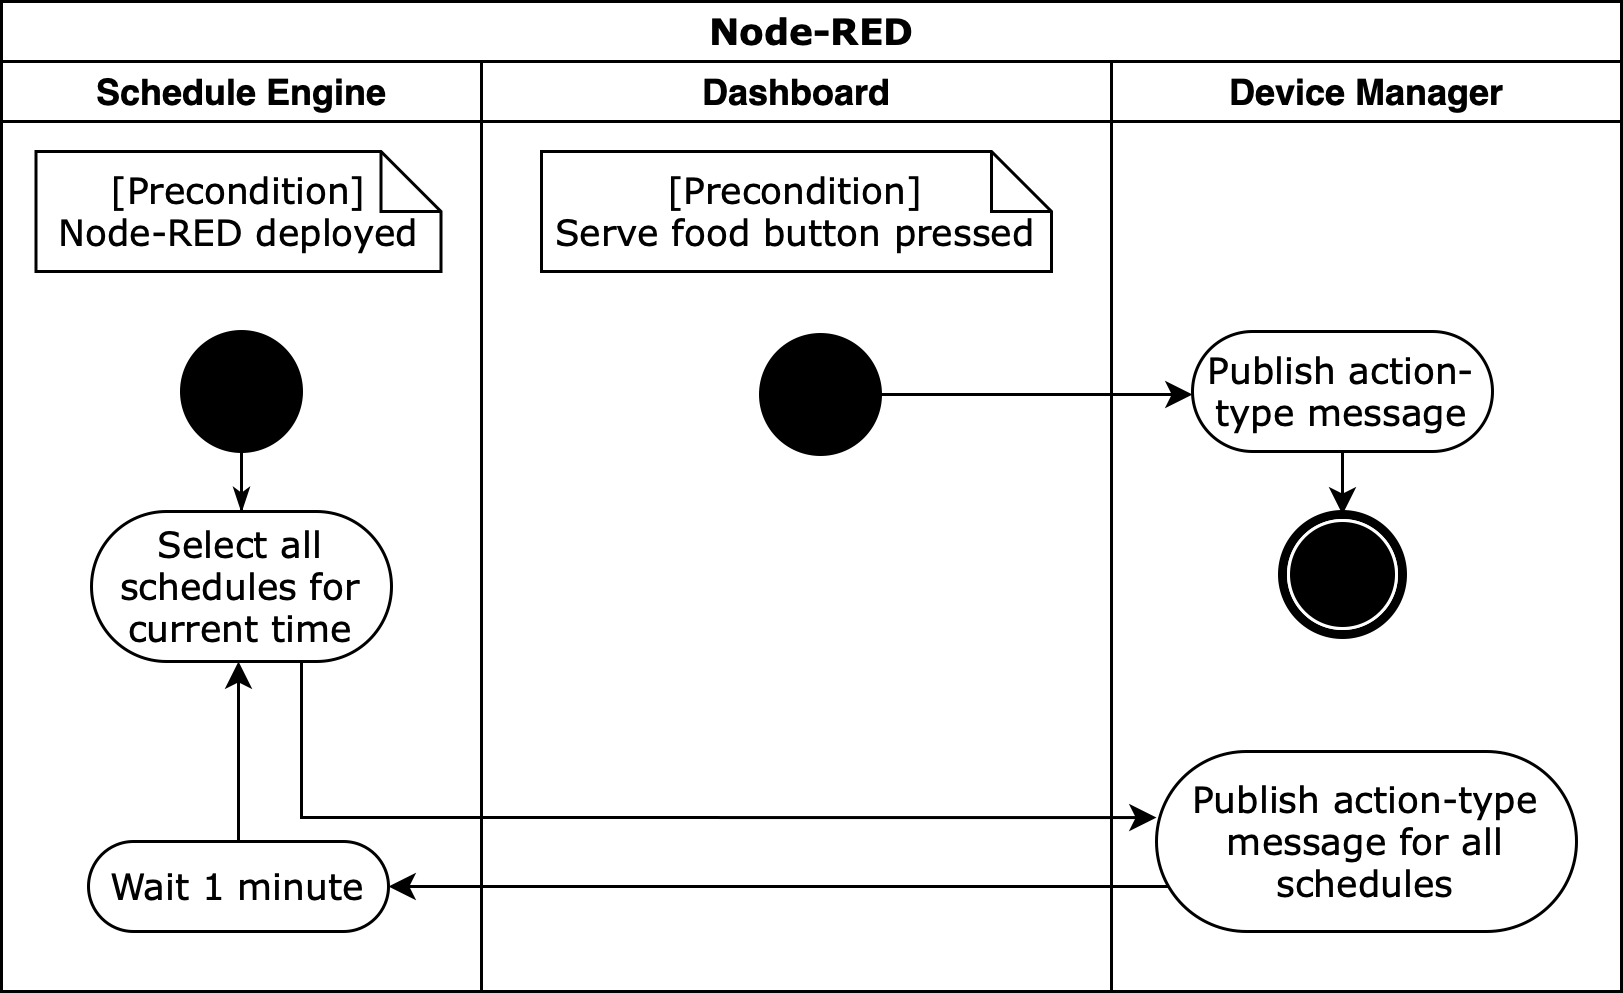
\includegraphics[width=0.5\textwidth]{publishActionMessage.png}}
\caption{Activity Diagram for Publishing Action Message.}
\label{fig}
\end{figure}
Activity diagram for Publishing action message is shown in figure ?
% `publishActionMessage.png`
. Publishing action message has two entry point: When serve button is pressed by user, and when Node-RED flow is deployed. When serve button pressed by user, event is tossed to the Device Manager block, and publish action-type message with serving amount is stored to message payload. Second entry point is to publish action-type message according to schedule. After Node-RED flow is deployed, Schedule Engine selects all the schedule where schedule’s execution time matches with current time. And then, Schedule Manager publishes all the action-type messages that is stored in schedule with the help of Device Manager. Finally, after all the action-type messages are published, Schedule Engine wait for another minute, and repeats selecting schedule procedure.

\hfill \break
\subsubsection{Receiving Error Message}
\begin{figure}[htbp]
\centerline{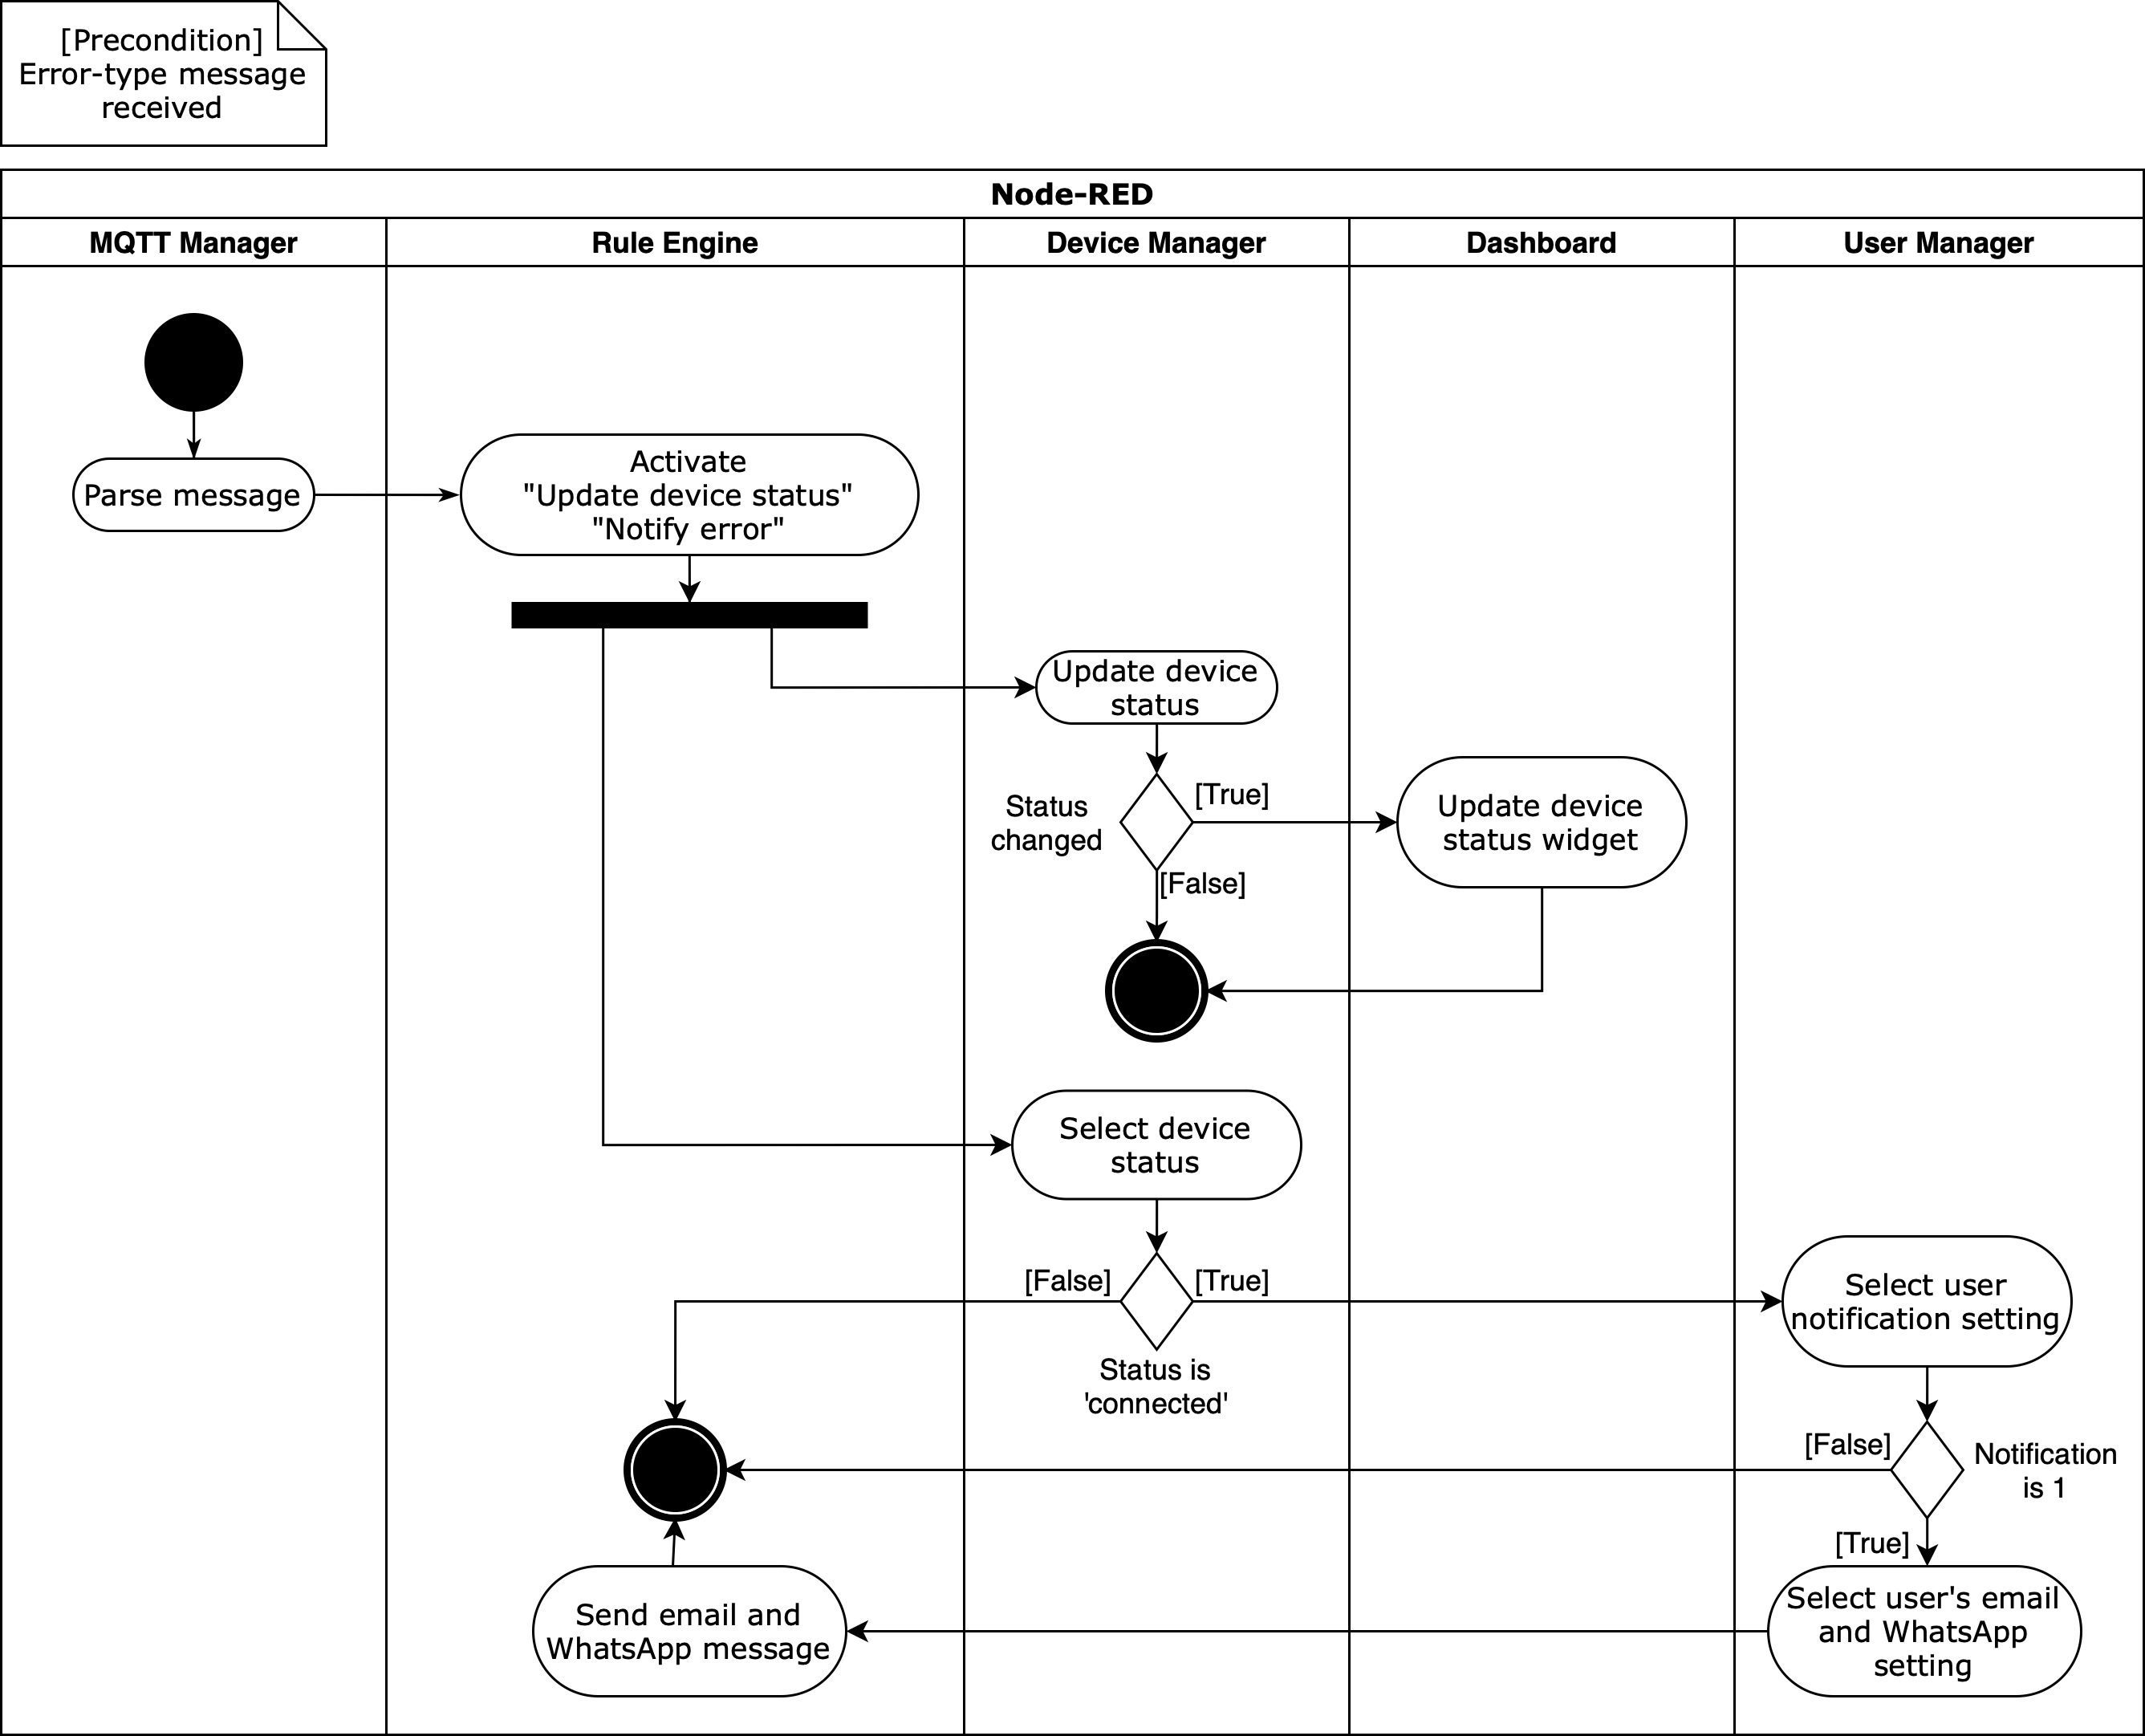
\includegraphics[width=0.5\textwidth]{errorMessageReceived.png}}
\caption{Activity Diagram for Receiving Error Message.}
\label{fig}
\end{figure}
Activity diagram for Receiving error message is shown in figure ?
% `errorMessageReceived.png`
. Similarly with the receiving scale message, error-type message is parsed in the MQTT Manager block and tossed to the Rule Engine block when platform receives it. After that, Rule Engine block activates two rules in parallel: Update device status, Notify error. To update the status of the device, Rule Engine block sends a signal to the Device Manager block. Device Manager block updates the status of the device to error, and sends the signal to the Dashboard block to update the device status widget only if status of the device is changed. To notify the error to the user, Rule Engine block sends a signal to the Device Manager block to check status of the device. As sending the notification message is done only if status of the device equals ‘connected’. Device Manager block ignores error when status of the device is not ‘connected’. After checking the device status, Device Manager sends a signal to the User Manager block to check the user setting for notification. In case of notification being set to 0, User Manager block ignores the error as well. When notification is set to 1, User Manager sends the signal to the Rule Engine block, with user email and WhatsApp account setting. Finally, Rule Engine block sends email and WhatsApp message based on the user notification information.

\section{Implementation}
% subsection드가기 전에 한단락 할애
\subsection{Hardware}
%<장치 구현 사진 & 회로도 사진>%

\subsubsection{Device Setup}
Each device was configured to automatically execute Node-Red during Raspberry Pi booting using Process Manager 2 (PM2) library of NPM. ‘Inject node’ automatically starts all the device setup flow right after Node-RED is executed. First step for device setup is loading ‘settings.json’ file to connect to MQTT broker. It is done by ‘Read file node’, ‘Parse JSON node’. When MQTT client ID is not saved to ‘settings.json’ file, flow for getting client ID from platform server and saving it is executed with ‘HTTP Request node’ and ‘Write file node’. After all settings are loaded, MQTT dynamic connection and subscription takes place, which are introduced for new feature of release v2.1.0 \cite{b26}. The implemented Node-RED flow for device setup is shown in figure ?.

% `deviceCommonNodeRED.png`
\begin{figure}[htbp]
\centerline{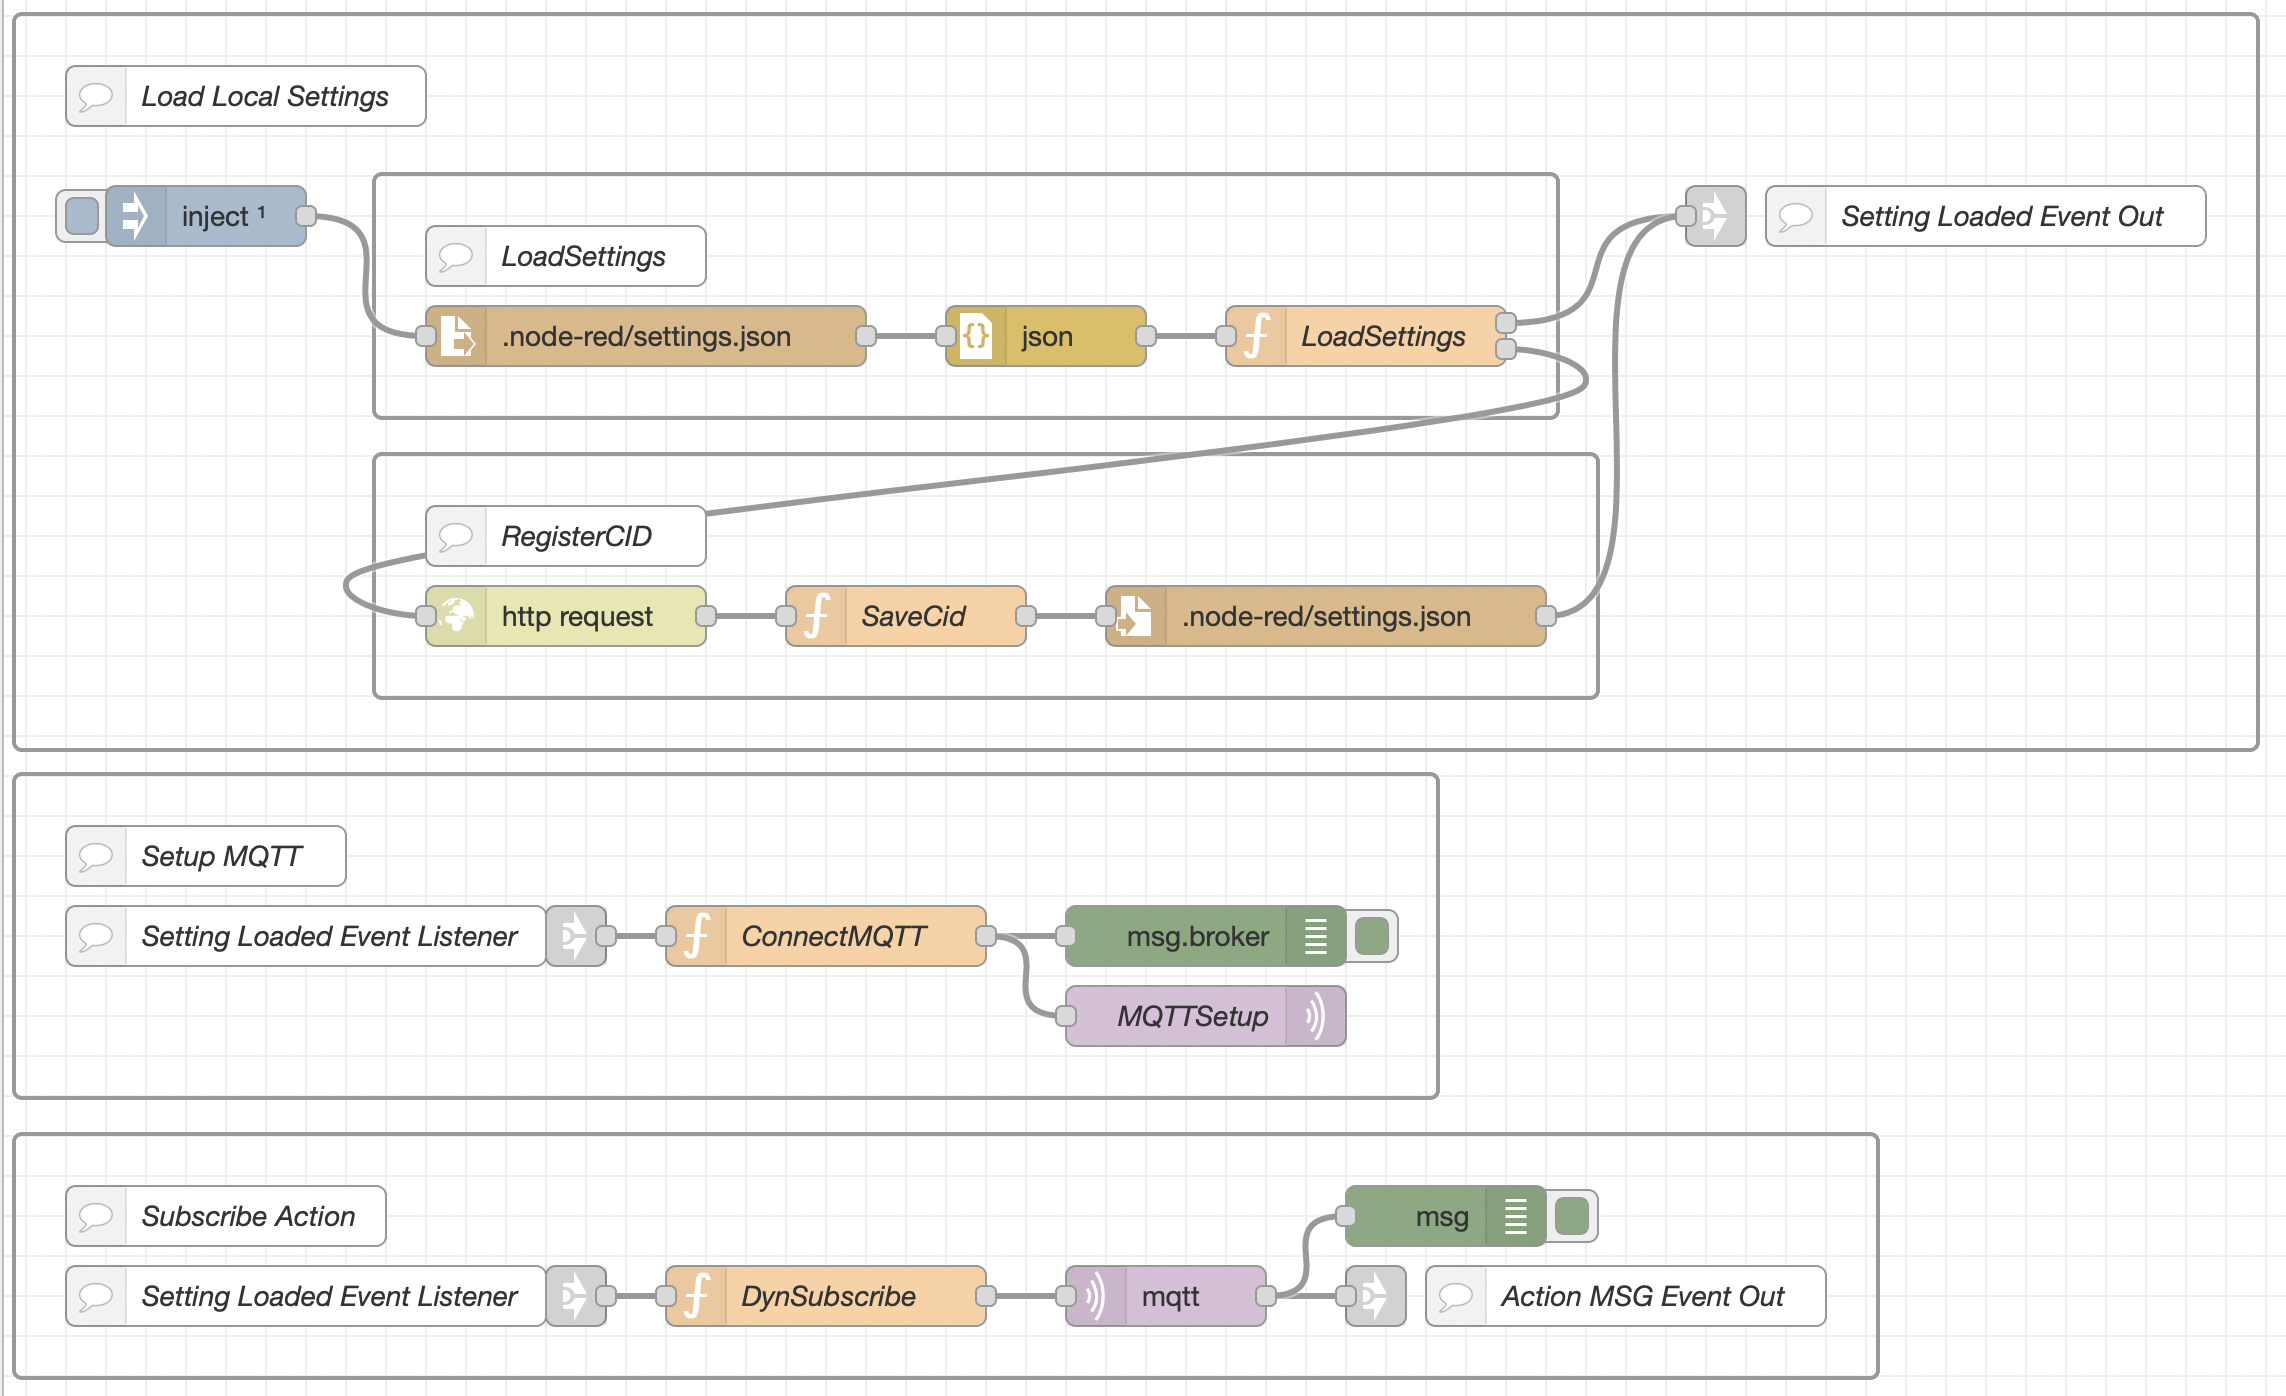
\includegraphics[width=0.5\textwidth]{deviceCommonNodeRED.png}}
\caption{Node-RED flow for device setup.}
\label{fig}
\end{figure}

\begin{figure}[htbp]
\centerline{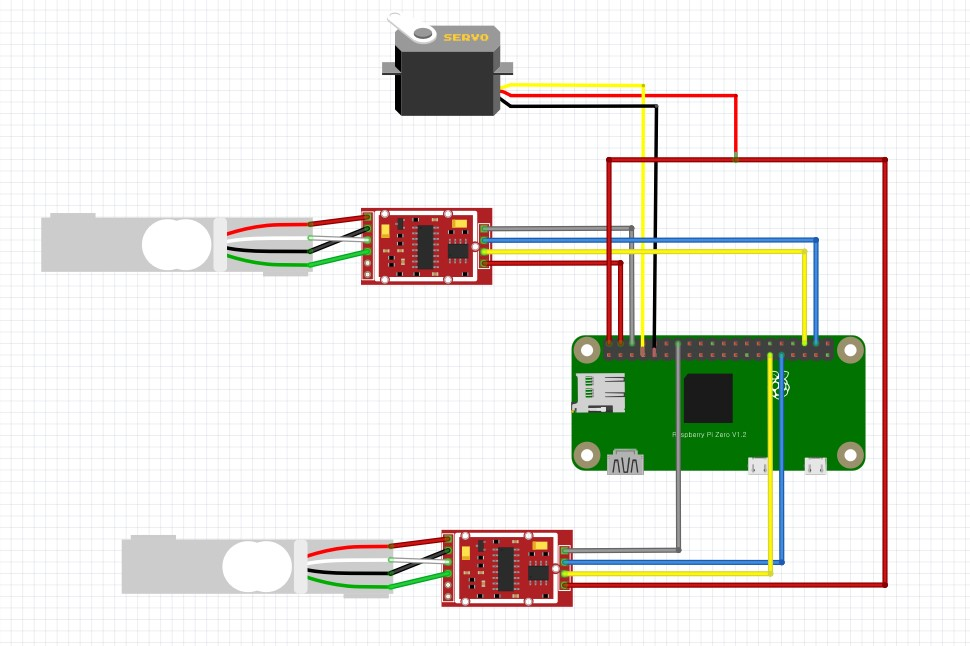
\includegraphics[width=0.5\textwidth]{feed machine circuit.jpg}}
\caption{Feed machine circuit diagram.}
\label{fig}
\end{figure}

\begin{figure}[htbp]
\centerline{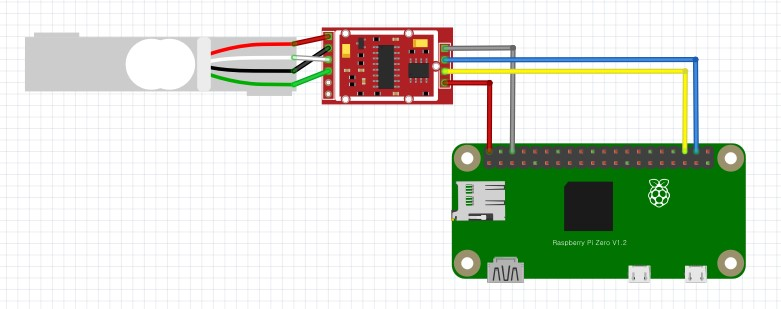
\includegraphics[width=0.5\textwidth]{water supplier circuit.jpg}}
\caption{water supplier circuit diagram.}
\label{fig}
\end{figure}

\begin{figure}[htbp]
\centerline{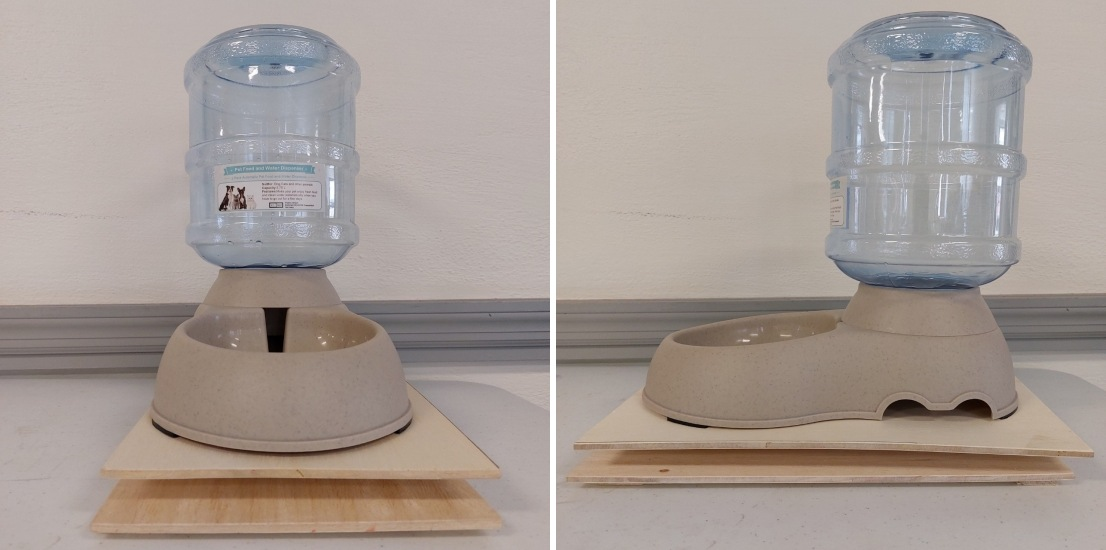
\includegraphics[width=0.5\textwidth]{Feed Machine.jpg}}
\caption{Feed machine device.}
\label{fig}
\end{figure}

\subsubsection{Feed Machine}
The feed machine uses 2 load cells, and each of the load cells measures the weight of the bowl
and the container. Exec node in Node-RED is used to execute the python file to use the
measurement using loadcell. At this time, the code is executed as a spawn to continue weighing
and uses a smooth node to provide the data flexibly (for example, calculating the average of 5
measurements). Then the error detector switch node is used to check for errors. If there are no
errors, the message set is taken into action for MQTT message publishing. The measurement of
the bowl and the container are each published as .../scale/bowl and .../scale/container form as the
topic so that it is provided to the client who has subscribed to that topic.
The user can use the dashboard to schedule a time for feed or the amount of feed. To do this, a
servo motor is attached to the container device to open and close the door of the container to
supply food to the bowl. The user’s initial input or the scheduled feeding’s action message is led
to the device action flow through the common flow’s action MSG event out node. Then the
bowl’s weight and the user’s input of desired food weight are combined to one message. It is sent
to a loop node and if the index is 0 and the bowl weight is less than the user’s input, the
container’s servomotor opens the door to provide food. It continues to compare the two weights,
the bowl weight is measured, and the payload of the message sent is continuously updated.
During the loop, when the bowl weight becomes bigger than the user’s input, the loop ends and
the servo motor closes the door and ends feeding.

\begin{figure}[htbp]
\centerline{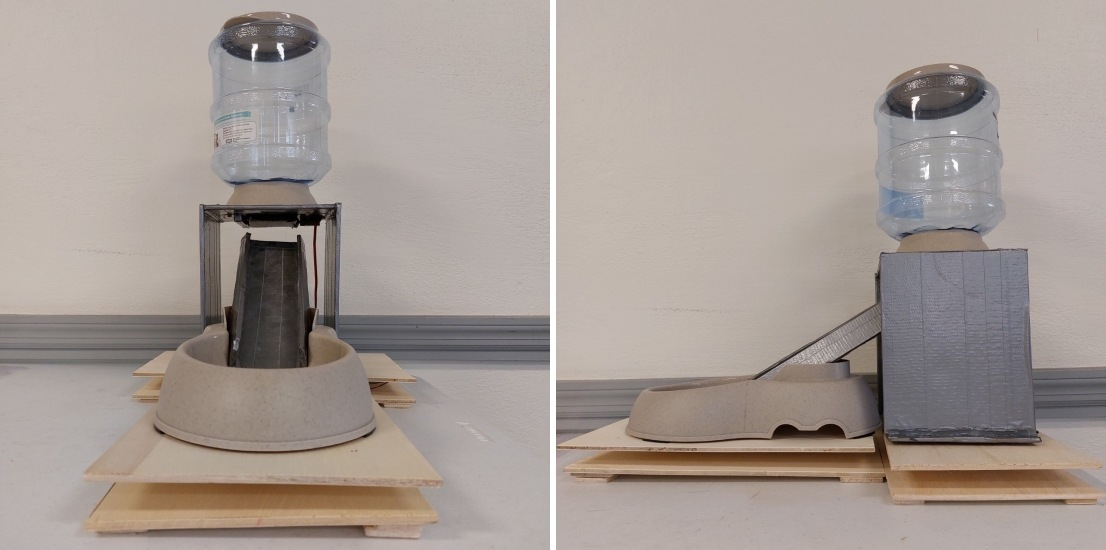
\includegraphics[width=0.5\textwidth]{Water Supplier.jpg}}
\caption{Water supplier device.}
\label{fig}
\end{figure}


\subsubsection{Water Supplier}
The water supplier uses one load cell to weigh the water. The process of measurement of the
weight is the same as the feed machine. The measured weight is published as ../scale/water form
of topic, and it is provided to the client who has subscribed to that specific topic.

\begin{figure}[htbp]
\centerline{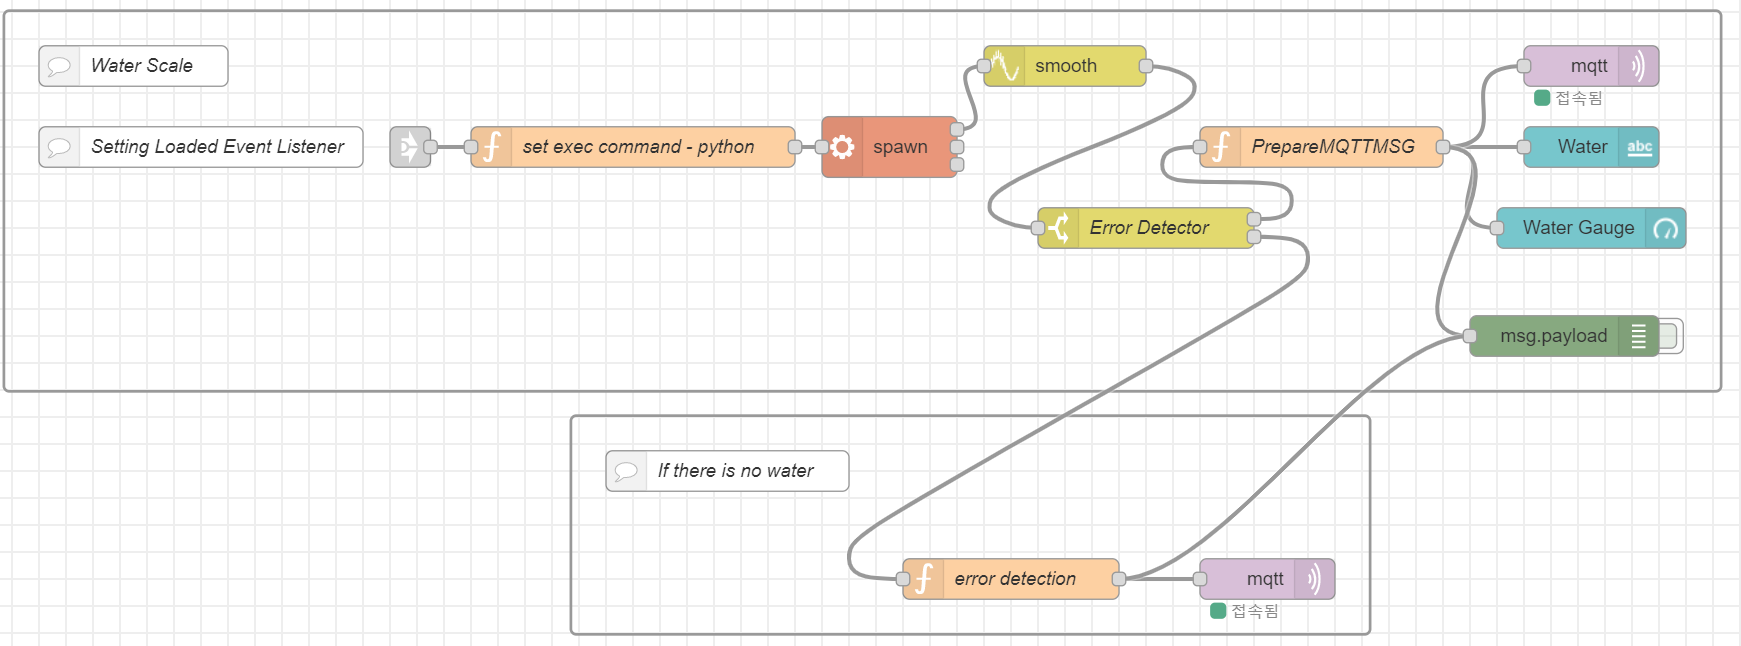
\includegraphics[width=0.5\textwidth]{Water Supplier Error Detection.png}}
\caption{Water Supplier Error Detection Flow.}
\label{fig}
\end{figure}

\subsubsection{Error Detection}
Each device measures the weight of the food and water left, and if the food or water is
insufficient it will send an error message to the platform server and check the user’s settings on
the platform server, and send a message to the user.

\subsection{Platform}
Platform for Petification uses cloud instance for deployment. On the cloud instance, Mosquitto, MySQL and Node-RED are installed and firewall, DNS and certificate for TLS/SSL communication are configured for networking. In the Node-RED, 7 blocks are implemented as 7 flows. The screenshot for implemented Node-RED flow is shown in Figure 19.

\begin{figure}[htbp]
\centerline{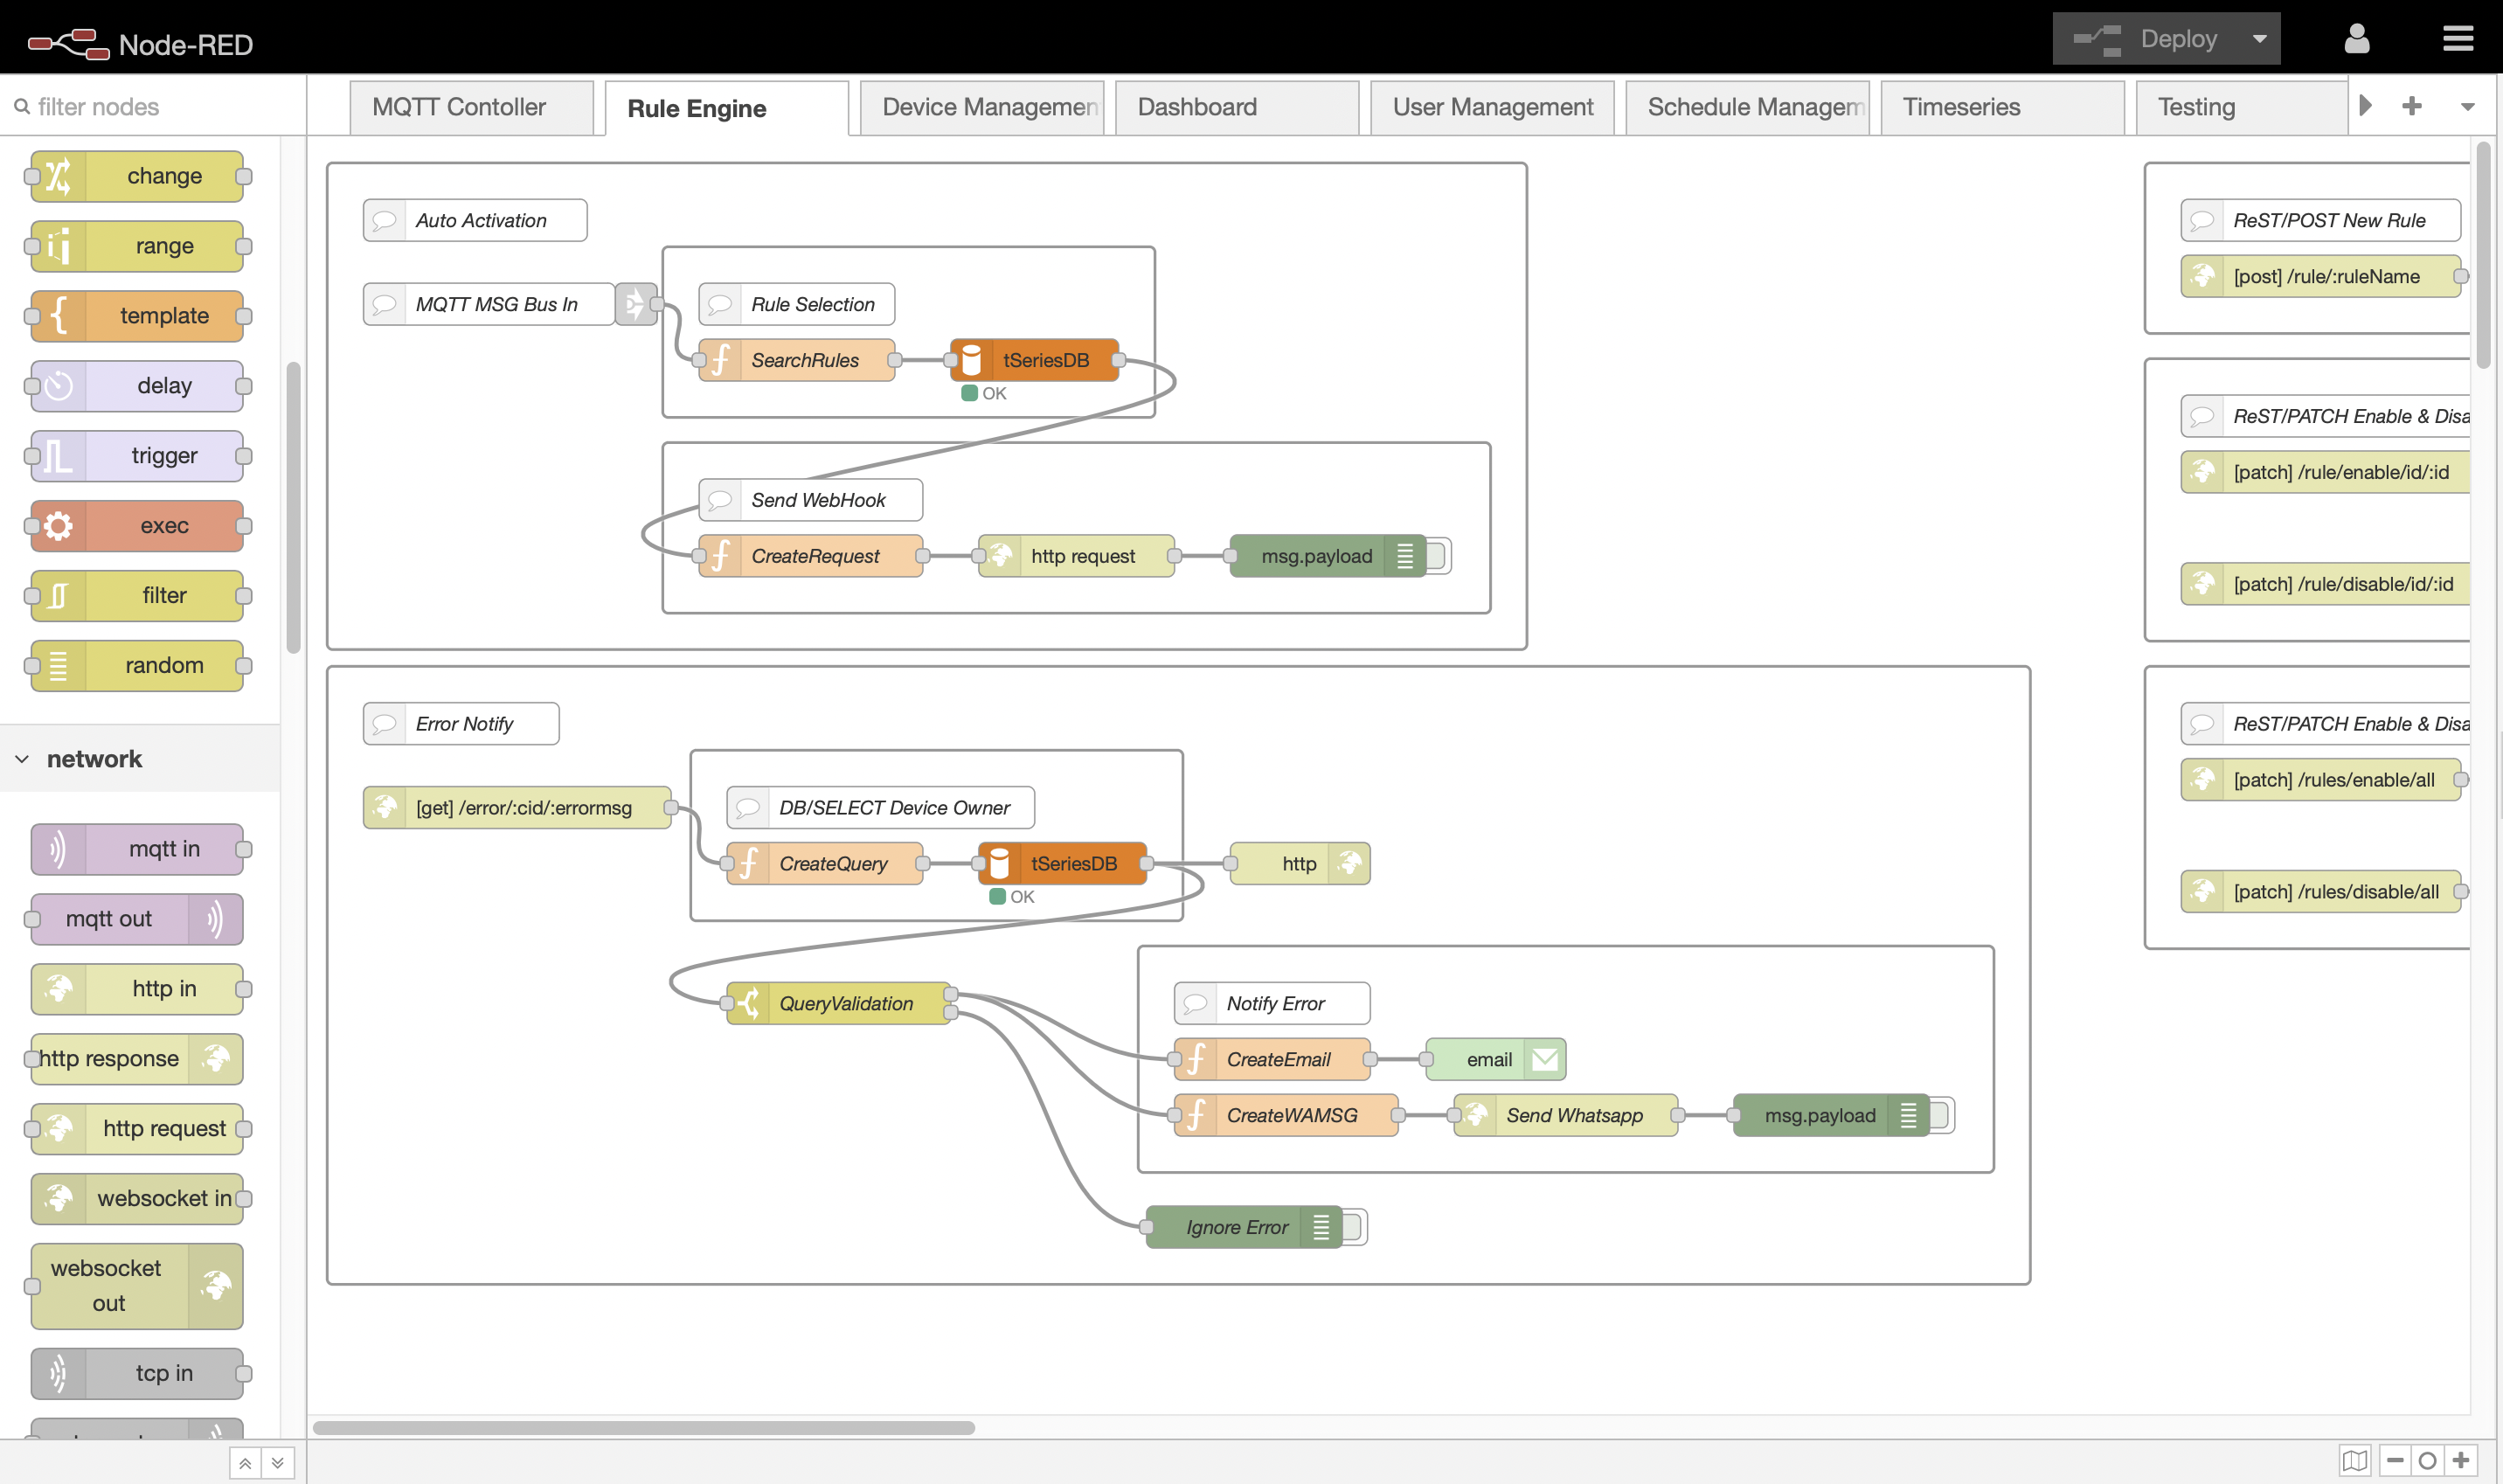
\includegraphics[width=0.5\textwidth]{platformImpl.png}}
\caption{Screenshot for Node-RED flow of platform.}
\label{fig}
\end{figure}

%%%%%%%%%%%%%%%%%%%%%%%%%%%%%%%%%%%%%%%%%%%%%%%%%%%%%%%%%%%%%%%%%%%%%%%%%%%
\subsection{Dashboard}
Petification’s dashboard was implemented using ‘node-red-dashboard’, which provides a set of nodes to make a live data dashboard \cite{b19}.
Dashboard consists of three tabs: Feed Machine tab, Water Supplier tab, and User Settings tab. \\

\subsubsection{Feed Machine tab}
In Feed Machine tab, Device Information widget, Feed Machine Statistics widget, and Serve Food widget is provided. As all the functionalities this tab provides are device specific, selecting device is included in Device Information widget. Thus, all the devices which user has and device type is water supplier are inquired from database, and they are displayed as a dropdown. Also, status for the selected device is provided in text and LED-shaped icon. The color of the LED-shaped icon changes to green when the device is connected, red for disconnected status, and yellow for error status. In Feed Machine Statistics widget, Remaining amount of food and container and food consumption is provided. Remaining amount of food bowl and container is displayed as gauge and food consumption is displayed as line graph. In Serve Food widget, user input interface is provided to publish feed serving action by button. Serve Food widget also provides the interface for automatic food feeding (scheduled feeding). User can see all the feeding schedules in the table format, add new schedule by user input interface, and delete the existing schedule by clicking row of the table. Figure 20
% `feed_machine_ui.png`%
shows the screenshot of implemented Feed Machine tab.

\begin{figure}[htbp]
\centerline{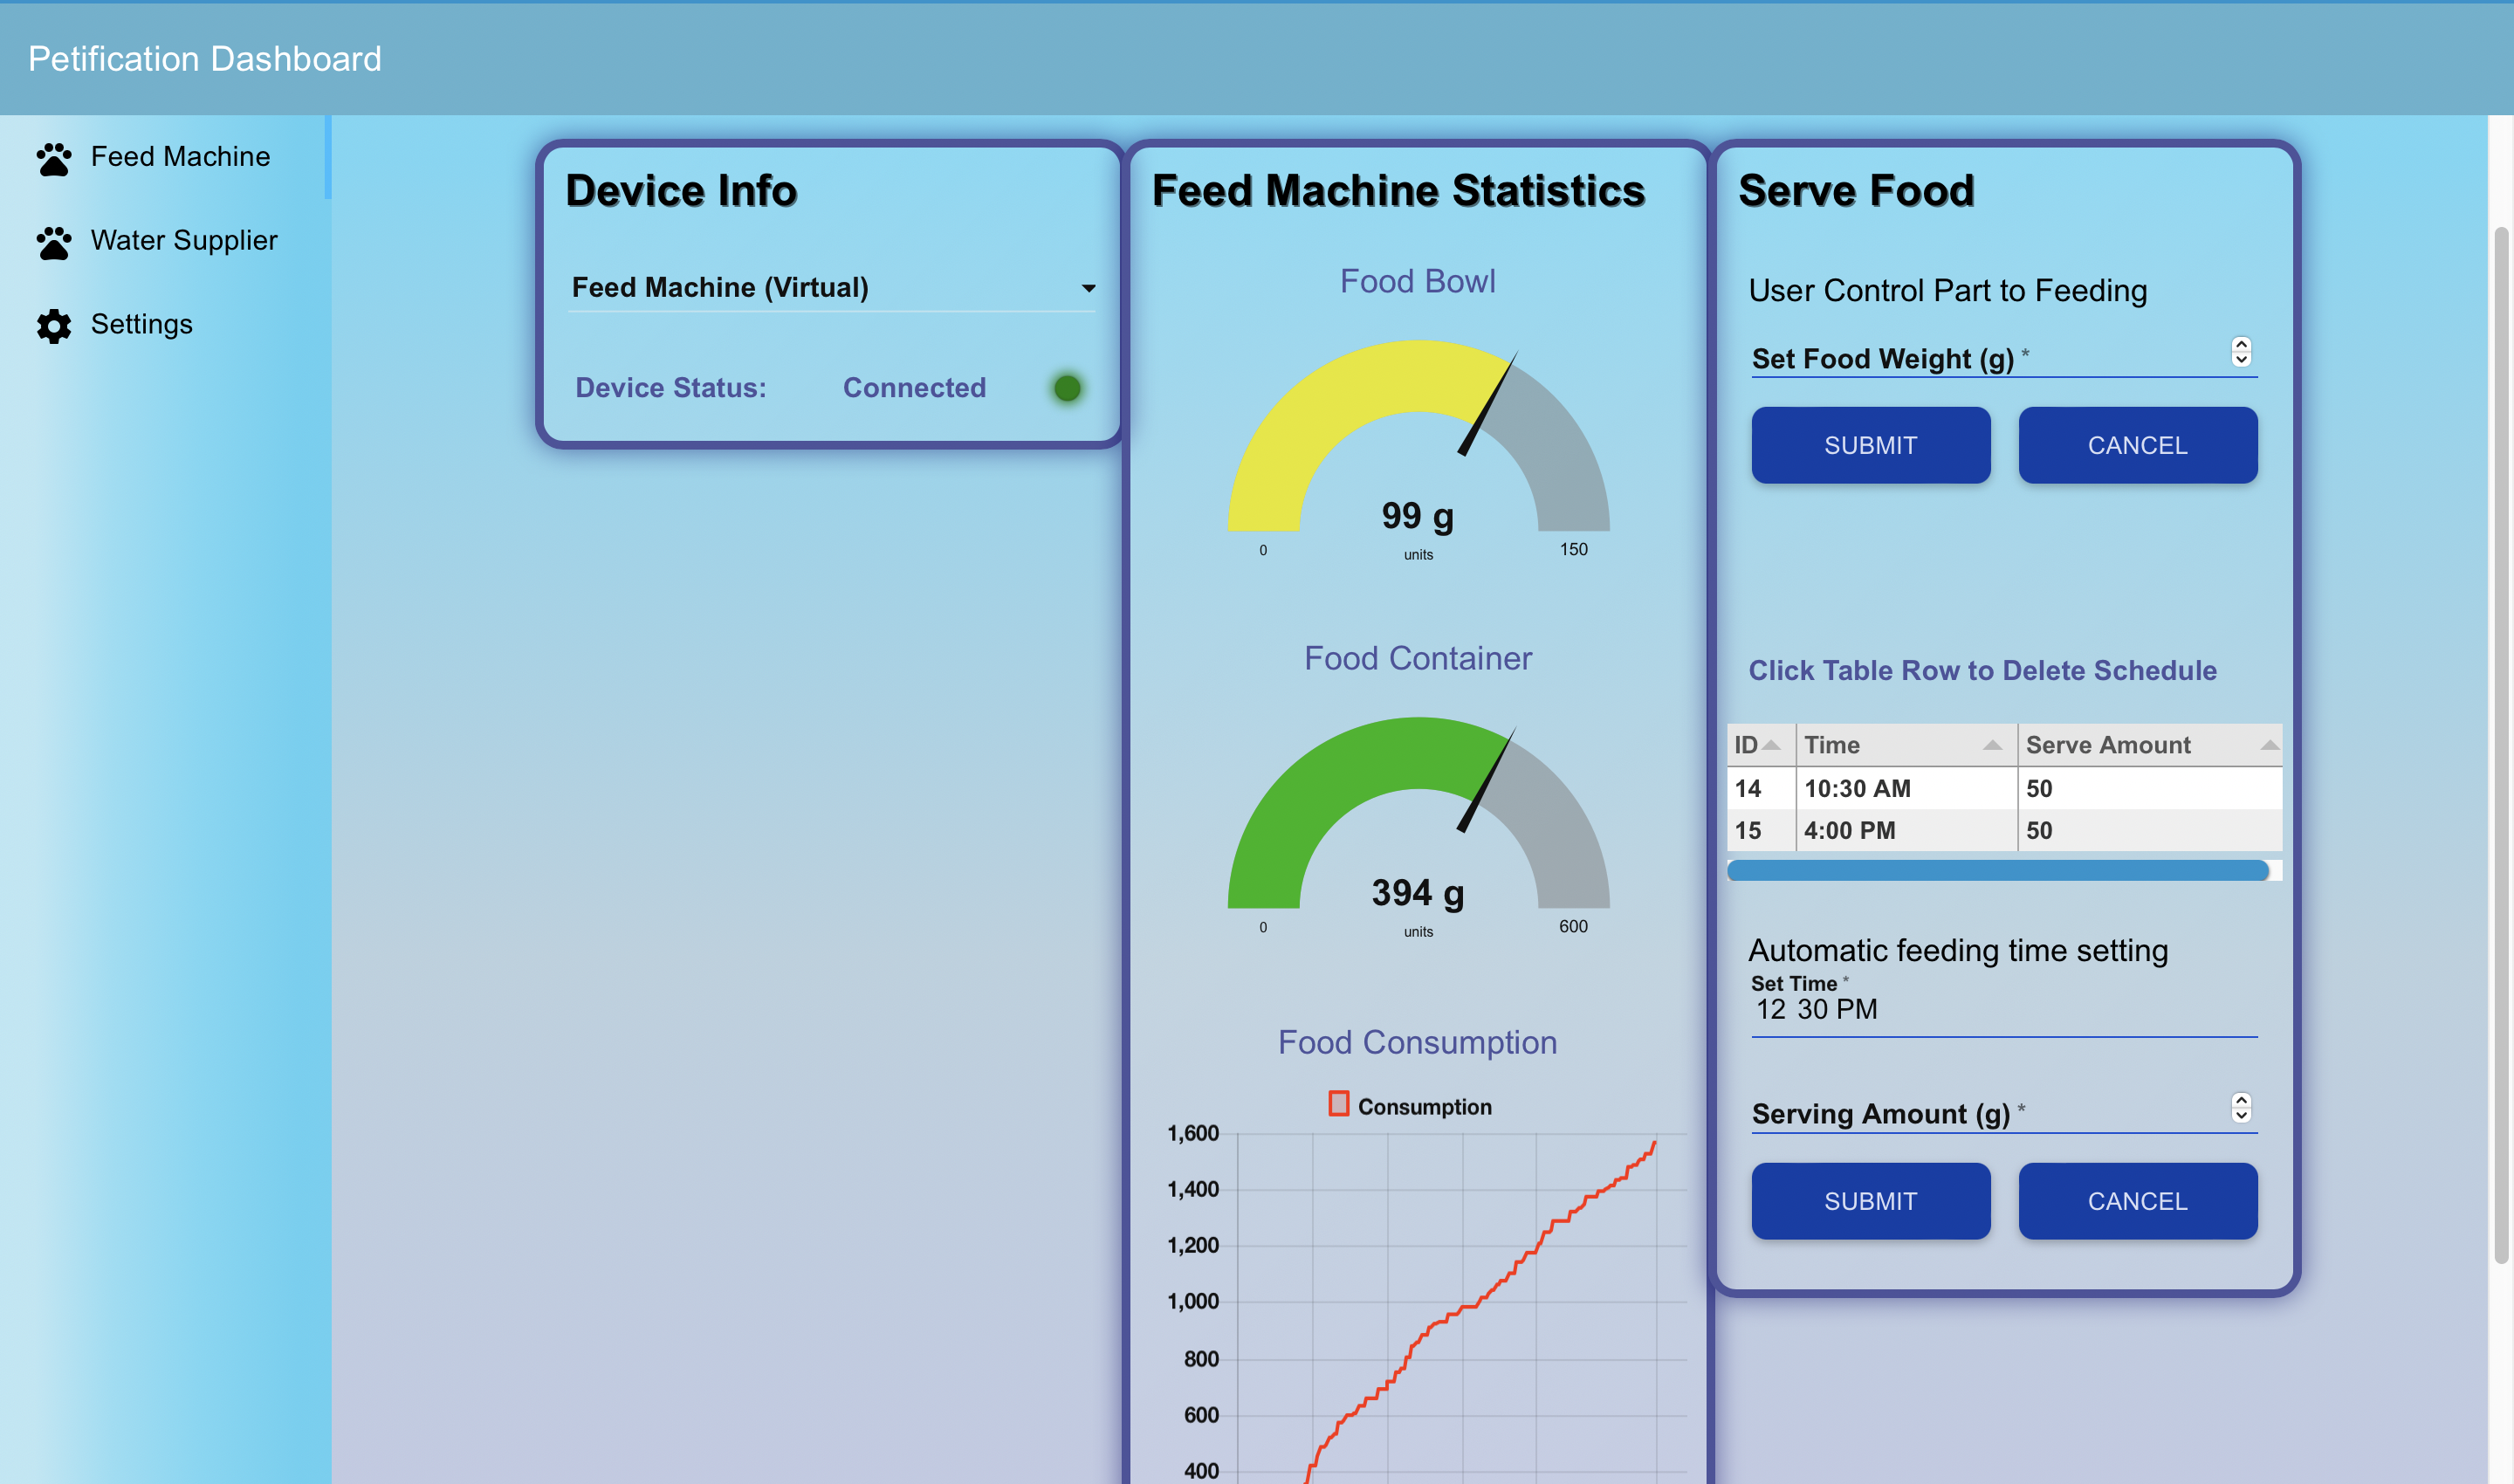
\includegraphics[width=0.5\textwidth]{feed_machine_ui.png}}
\caption{Screenshot for Feed Machine tab.}
\label{fig}
\end{figure}
% `This figure should be replaced with real device selected screen shot.`

\subsubsection{Water Supplier tab}
Similarly with the Feed Machine tab, Water Supplier tab provides two widgets: Device Information widget and Water Supplier Statistics widget. The mechanism for each widget is identical with the Feed Machine tab. Figure 21
% `water_supplier_ui.png`
shows the screenshot of implemented Water Supplier tab.

\begin{figure}[htbp]
\centerline{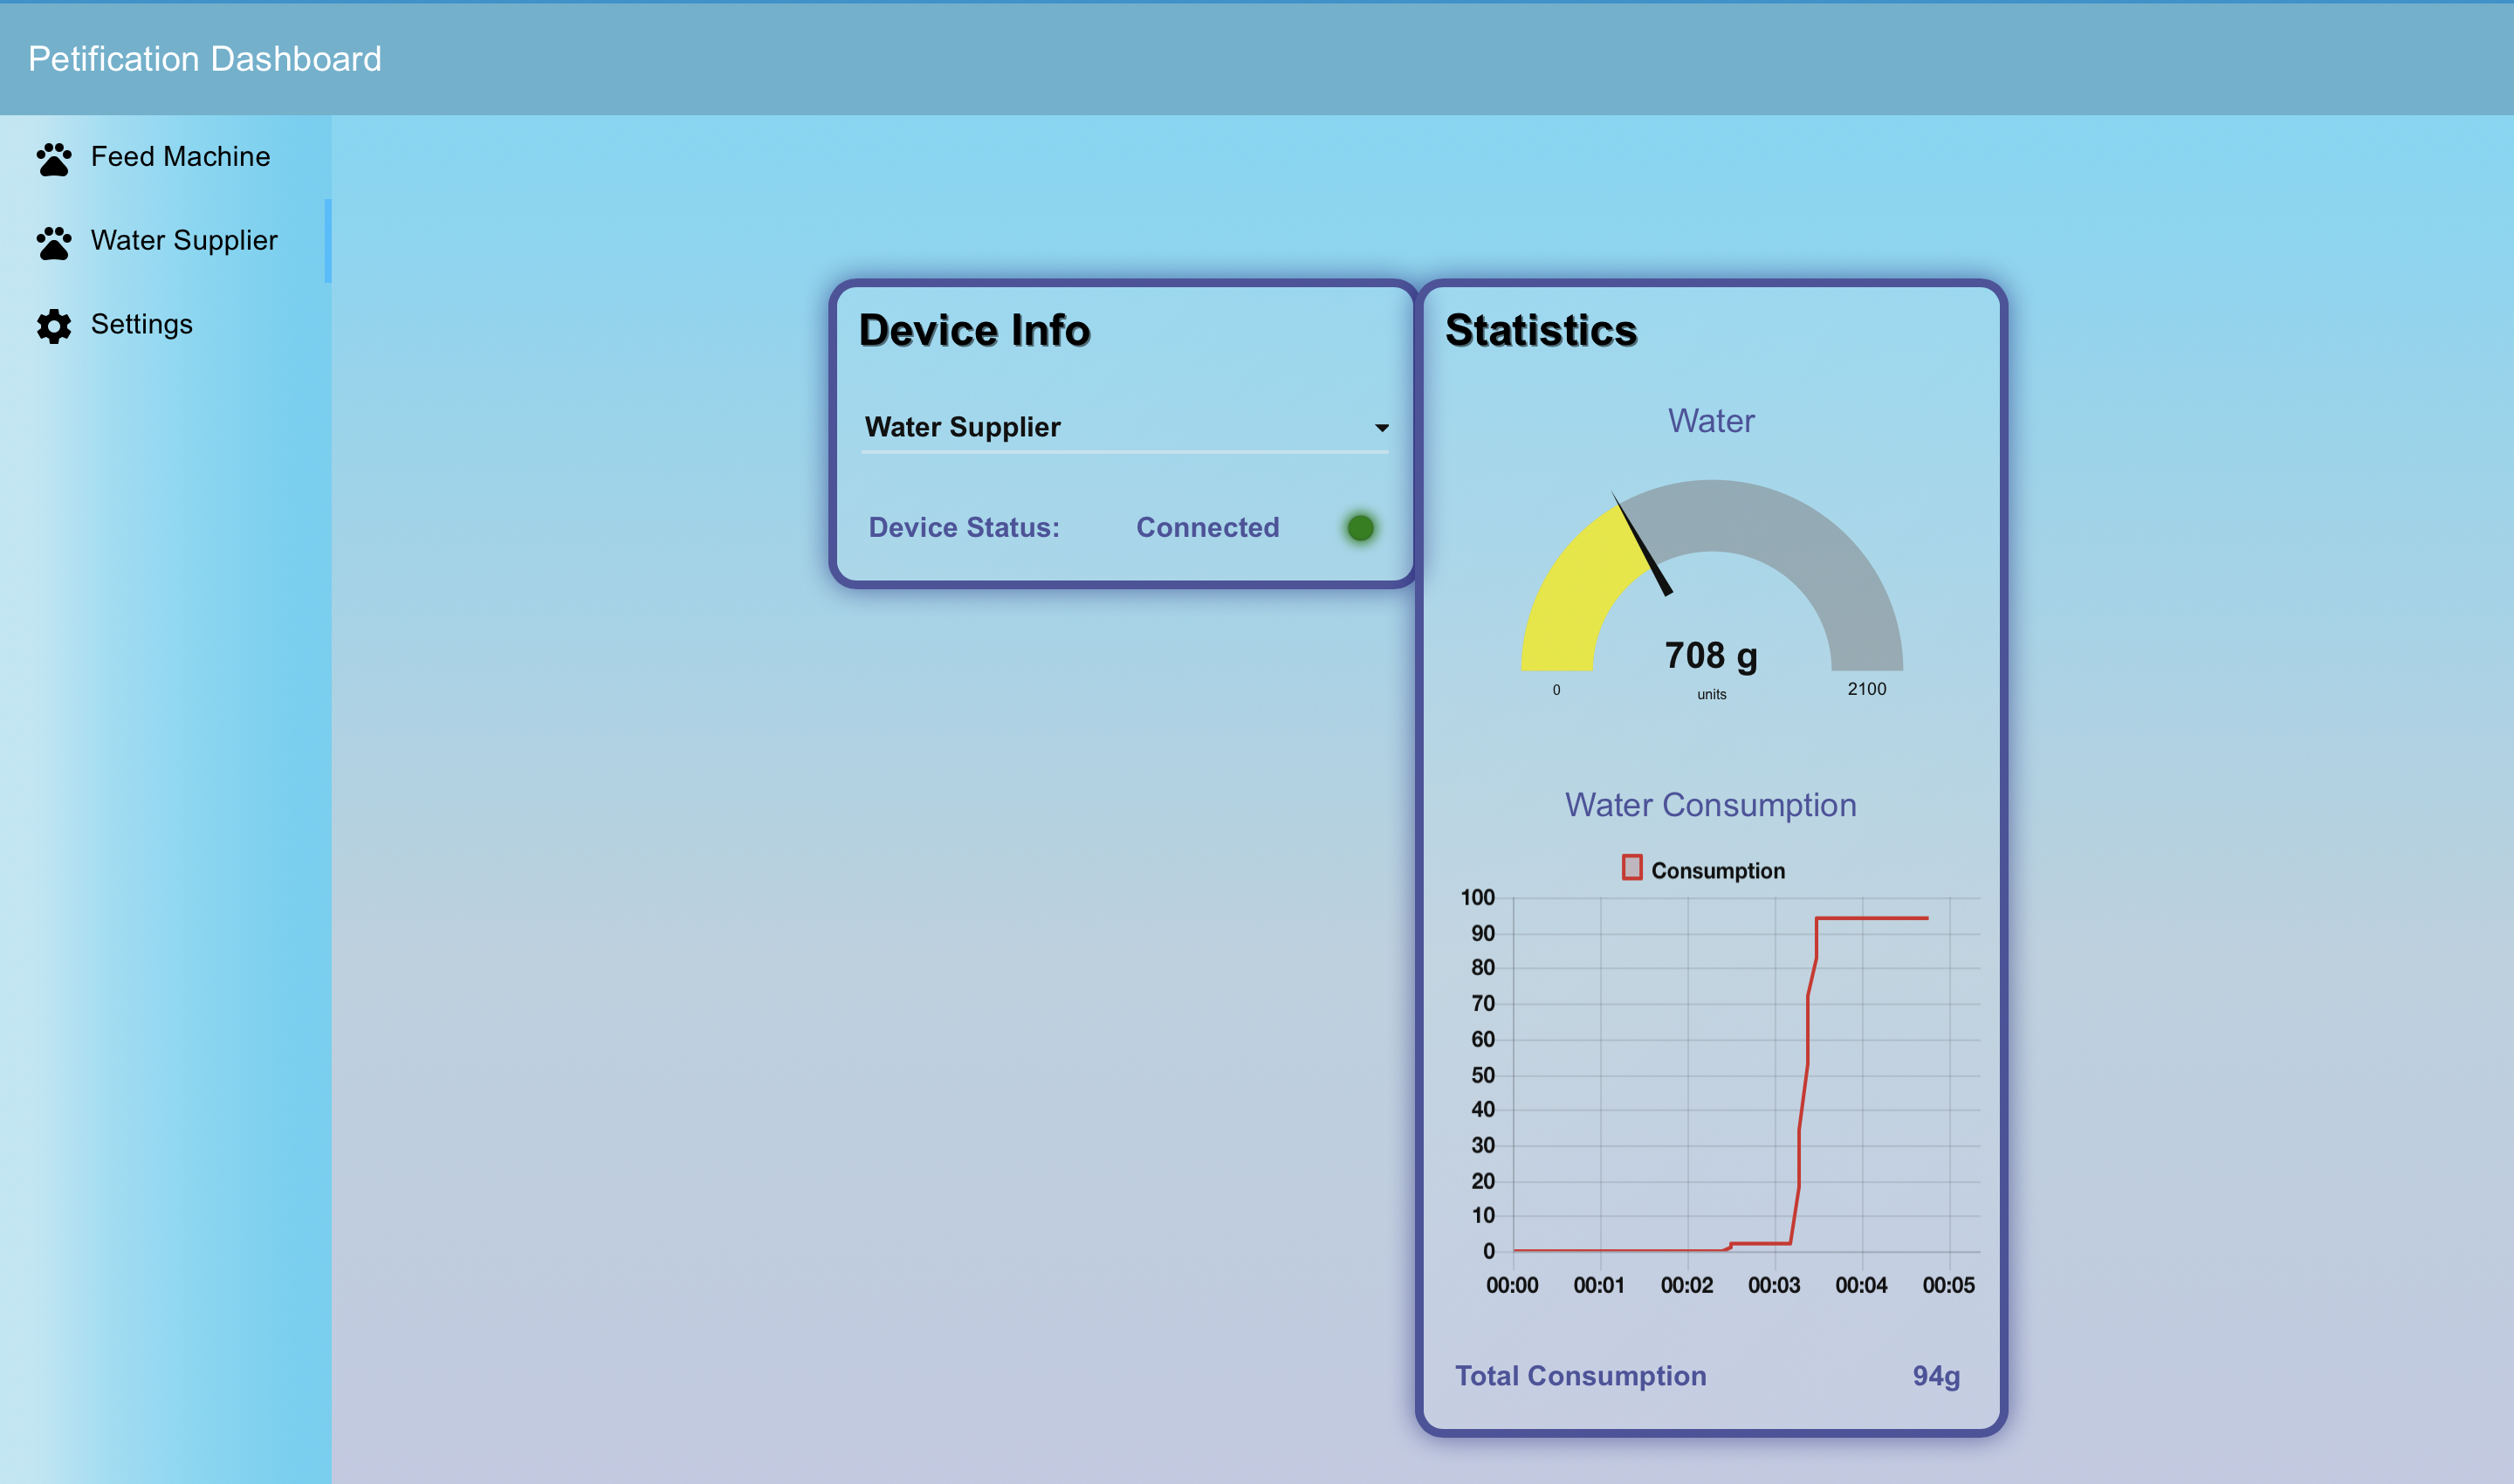
\includegraphics[width=0.5\textwidth]{water_supplier_ui.png}}
\caption{Screenshot for Water Supplier tab.}
\label{fig}
\end{figure}

\subsubsection{User Settings tab}
The main purpose for User Settings tab is to manage user information and the settings. This tab provides five widgets: User Information widget, Timezone settings widget, Notification settings widget, E-Mail address settings widget, and WhatsApp settings widget. Handling user information is the main functionality for User Information widget. User information is defined with two value: token and username. Each user account has unique token and username, and token is to authorize user when handling HTTP request. For username, it is used when MQTT Broker block authenticates user. Thus, in order for users to use all the features petification provides, the user must be registered to petification with valid token and username. In User Information widget, user can see the token and username, and by typing token to the user input interface, user can change the user account.
\indent In order to support global users, Timezone settings widget is included to the tab. As all the times that platform uses and database stores uses Coordinated Universal Time (UTC) timezone, converting time of the user to the UTC is necessary. Notification settings widget, E-Mail address settings widget, and WhatsApp settings widget is to control error notification. Users can turn notifications on and off with the Notification settings widget and decide which accounts receive email and WhatsApp messages. Figure 22
% `user_settings_ui.png`
shows the screenshot of implemented User Settings tab.

\begin{figure}[htbp]
\centerline{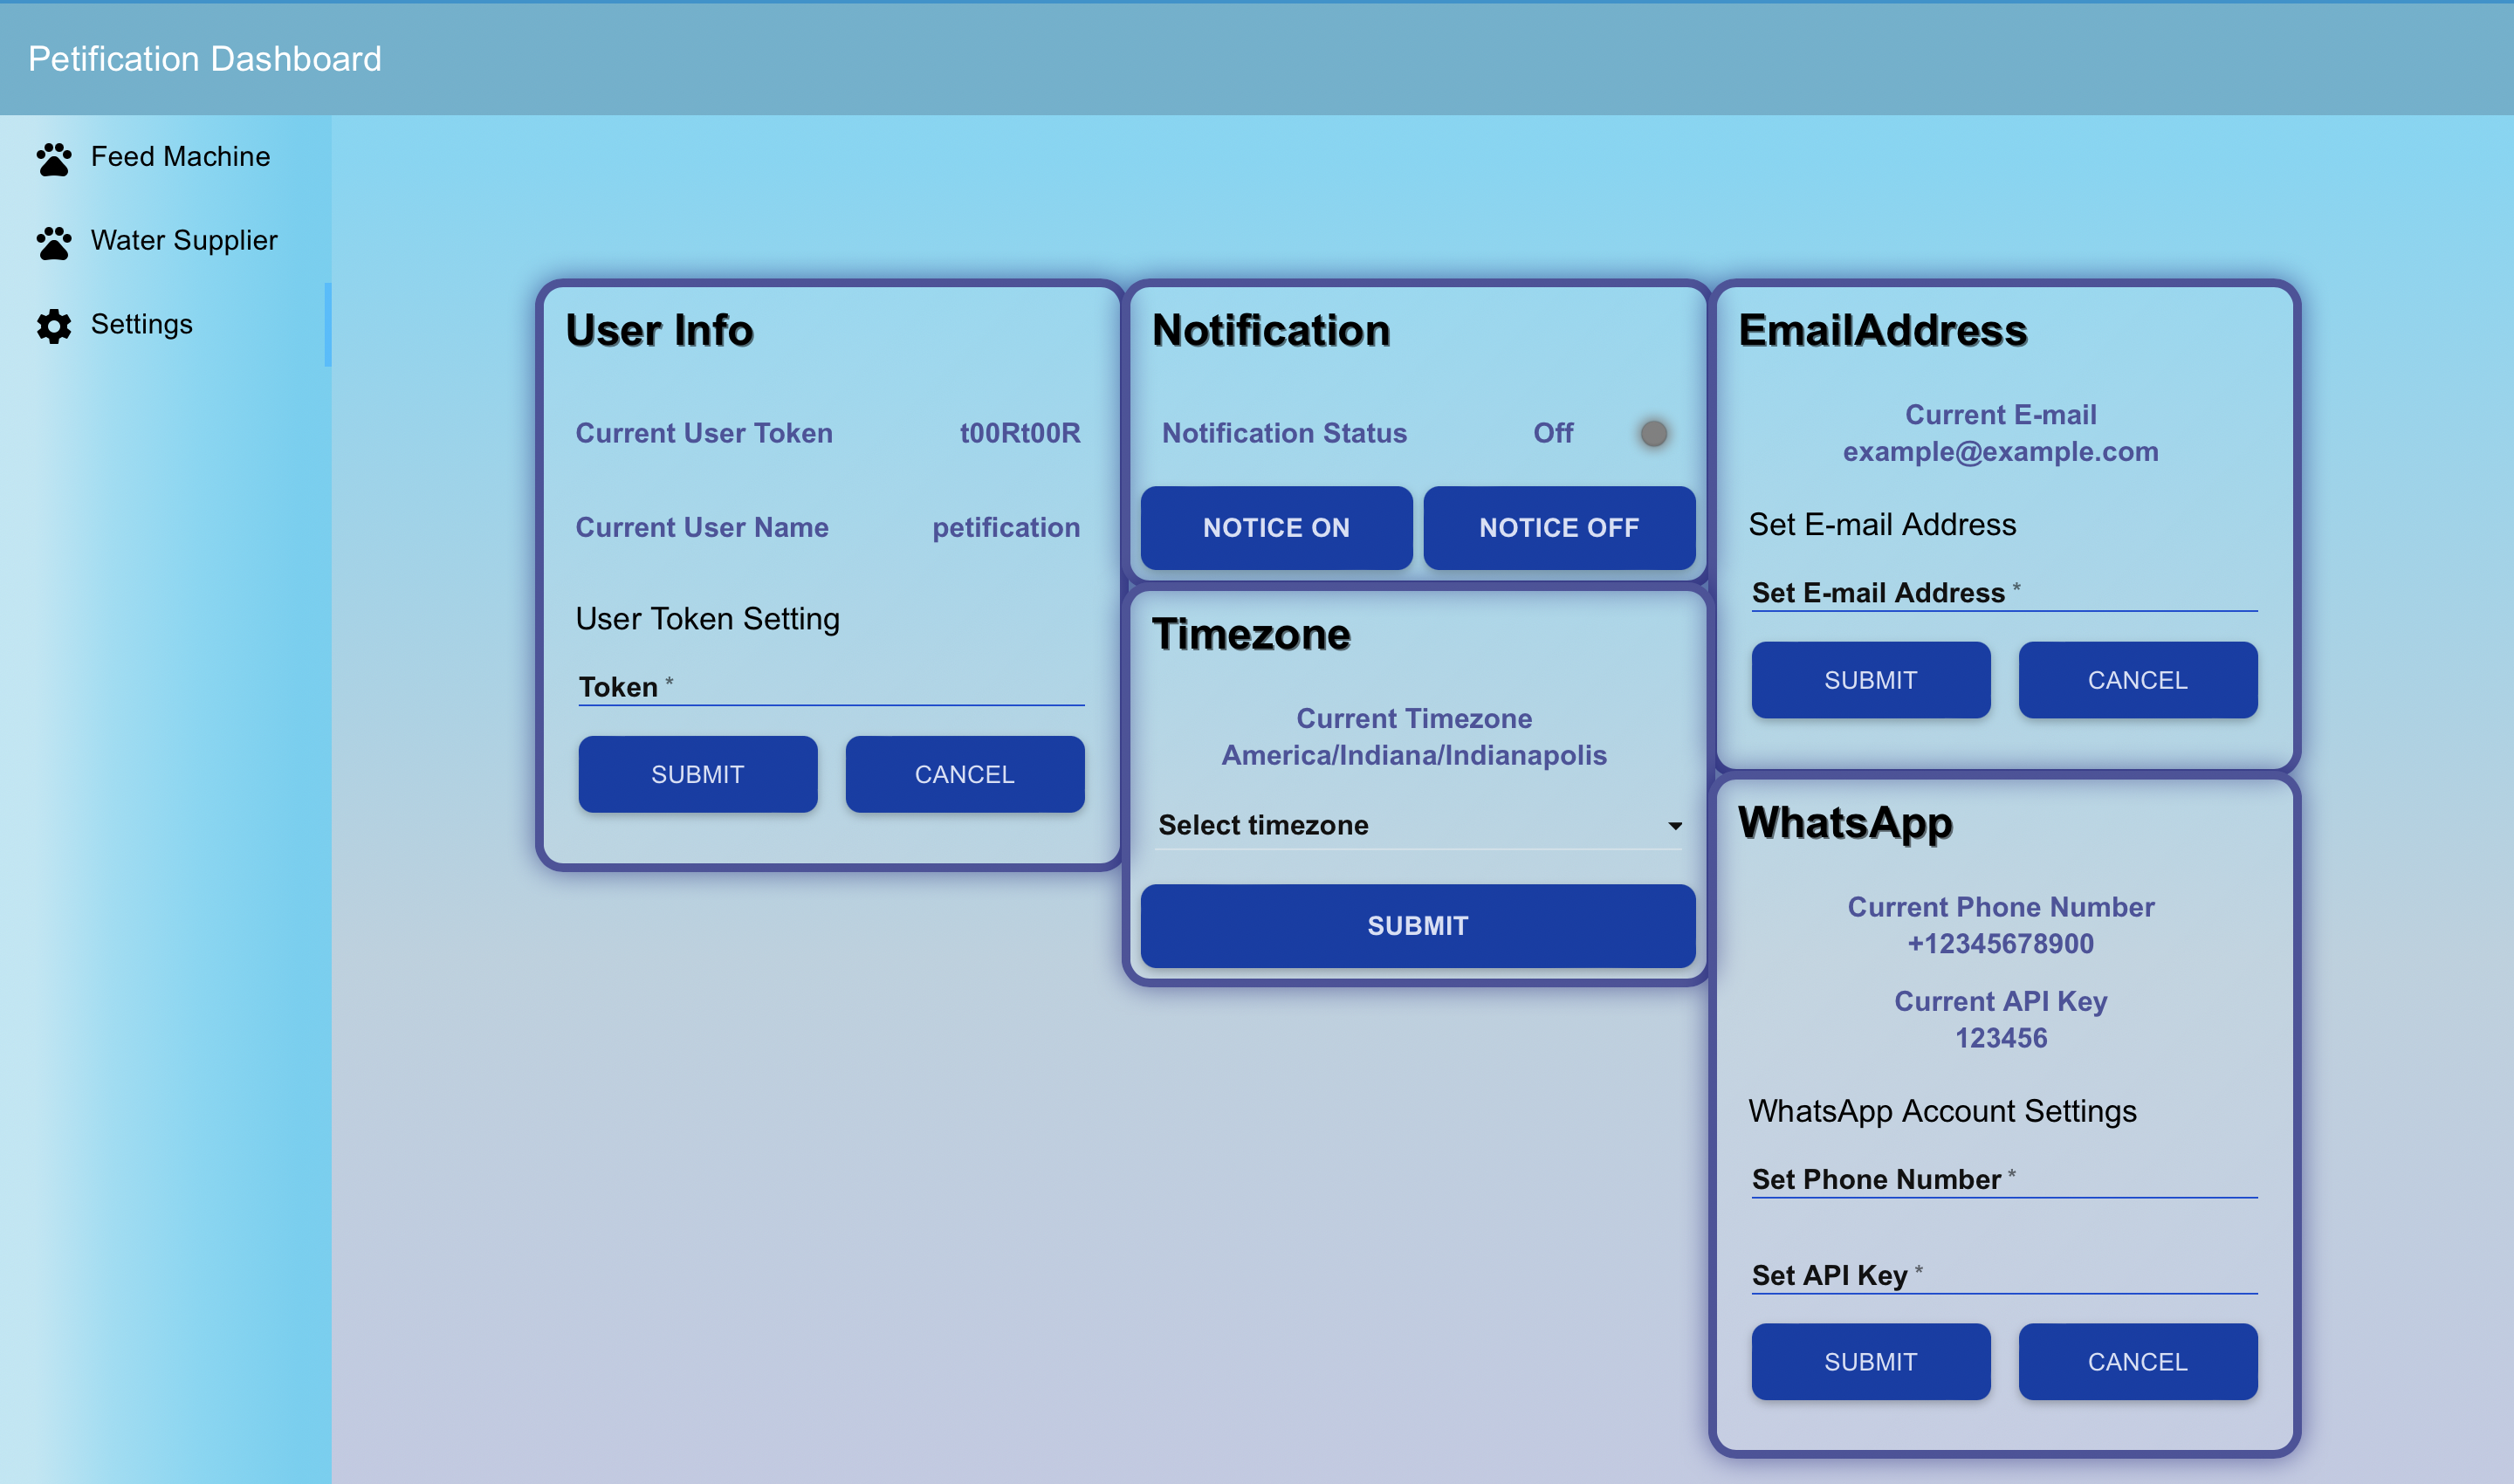
\includegraphics[width=0.5\textwidth]{user_settings_ui.png}}
\caption{Screenshot for User Settings tab.}
\label{fig}
\end{figure}
%%%%%%%%%%%%%%%%%%%%%%%%%%%%%%%%%%%%%%%%%%%%%%%%%%%%%%%%%%%%%%%%%%%%%%%%%%%%%%%%%%%%%%%%%%
\section{Experiment}
% Experiment에서는 컨테이너 높이에 따라 나오는 양이 다른지 실험 해봐야 할 듯 >> 열리는 크기는 똑같으니깐 원하는 양을 맞추면 시간을 다르게 해야함 >> 이때 열리자 마자 닫히게 하면 막히는 경우가 많았으니깐 디바이스 앞에 보강 하던 아님 최소 열리고 있어야하는 시간을 측정해서 최소 줘야하는 양을 정해야 할 듯
Testing is conducted based on the results of implementation of the Petification IoT Platform. Testing is conducted only on quantitatively verifiable results, and a total of two cases are covered: accuracy testing of load cell weight sensors that have undergone calibration and scheduled/Manual Feeding testing. The results of the testing are conducted in an integrated connection environment including a Petification IoT platform that processes logic, a device that plays the role of sensing with an actuator, and a dashboard to check the results.

\subsection{Calibration Testing}
Calibration must be performed initially to use the load cell. 
In this study, the weight of 500ml bottled water was fixed at 500g for calibration. Thereafter, a total of 8 tests were performed using a load cell sensor in which calibration was completed, and the weight measurement results for 500, 1000, 1500, and 2000 (g) were confirmed.

\begin{figure}[htbp]
\centerline{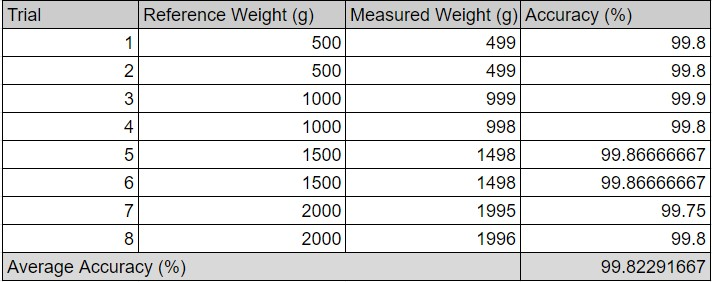
\includegraphics[width=0.5\textwidth]{Calibration_sheet.jpg}}
\caption{Screenshot for User Settings tab.}
\label{fig}
\end{figure}

It was confirmed that the average accuracy was 99.8\%, which resulted in high accuracy. Through this, it can be confirmed that the weight measurement error by the sensor hardly occurs in the result of subsequent testing.

\subsection{Scheduled / Manual Feeding Testing}

\begin{figure}[htbp]
\centerline{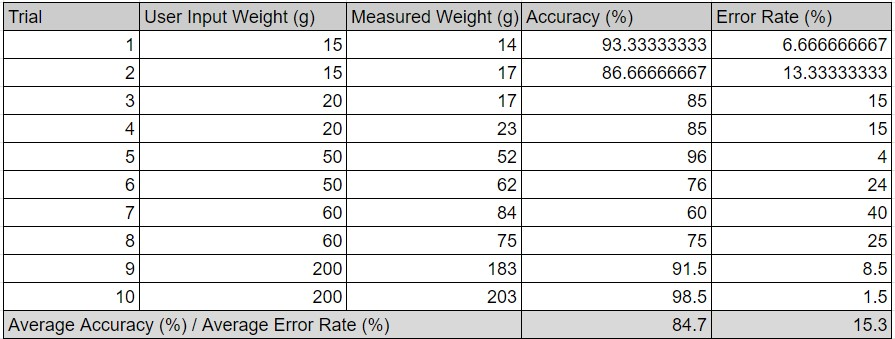
\includegraphics[width=0.5\textwidth]{Feeding_sheet.jpg}}
\caption{Screenshot for User Settings tab.}
\label{fig}
\end{figure}

Testing was conducted to see if the operation and result of the scheduled feeding and direct input feeding set by the user were well reflected.
For the weight values set in User input and Scheduled Feeding, the difference error from the weight value after feeding was tested.
As a result of the measurement, it was confirmed that 40\% of the highest error was found, and 1.5\% of the lowest error was found.
The reason for the error is that the amount of feed cannot be adjusted when feeding the device, which can be seen as a limitation of device. If the amount of feed in device can be supplemented, good results can be expected.

As a result of the testing, no functional errors occurred.
However, it is thought that it is necessary to supplement the adjustment of feed volume in device of Schedule / Manual Feeding Test, which is planned to be improved through a future plan.

\section{Conclusion}
This research paper is about the design and implementation of pet care IoT solutions via IoT
devices. For pet caring, IoT devices for feeding and providing water are implemented. For an
effective connection between the device and the user, the platform uses an MQTT Message
broker to receive data from the device, a database to store data, and Node-RED to execute and
visualize logic and data. The user interface was designed using Node-RED-dashboard and
WhatsApp was used to send notifications to the users via SNS to provide useful information and
services such as the remaining measurement, consumption, automatic/manual feeding, and
notification. In order to test the ability and the flow of the platform, we limited the device to feeding and water
supplying, however, users can use Node-RED to easily create a flow and add their own devices
to the platform. Furthermore, the user can design the database as they want since they’ve got
direct access to the database and create flows freely using Node Package Manager(NPM).
This research implemented a servo motor to provide food from the container to the bowl on the
feed machine. This resulted in limitations to control the amount of food being provided which led
to an error in the result value. A future recommendation to this research is to redesign the
device to weigh the food amount to provide just the amount that the user wants to fix the
problem rather than just using the servo motor to open and close the container door to provide
food. Through this research, we were able to show that the pet owners could utilize the
Node-RED-based platform that could collect data and create a visualization of the flow. 

The fact that this research encourages the users to easily design the platform’s services, the research is
not limited to the original platform’s ability. We look forward to a variety of IoT platform research
not just on pet care services.


\section{Acknowledge}
The authors would like to appreciate the support of Chungnam National University, Software-oriented university council, Purdue University and Institute for Information \& communication Technology Planning \& evaluation(IITP). Especially, the authors of this study are grateful to Professor Minsun Lee of Chungnam National University, Professor Eric and Tony of Purdue University, and Assistant Minji Lee for helping us participate in the project.

\begin{thebibliography}{00}
\bibitem{b1} 
M.  Hanson.  “Pet  Industry  Statistics”  spots.com.  https://spots.com/pet-industry-statistics/ (accessed Jan. 25, 2022). 
\bibitem{b2}
Accessed: Feb. 1, 2022. [Online]. Available: https://www.instructables.com/IOT-Pet-Feeder-Using-the-Blynk-Mobile-App-an-ESP82/
\bibitem{b3}
Accessed: Feb. 1, 2022. [Online]. Available: https://www.instructables.com/IoT-Pet-Feeder/
\bibitem{b4}
T. Sangvanloy and K. Sookhanaphibarn, "Automatic Pet Food Dispenser by using Internet of Things (IoT)," 2020 IEEE 2nd Global Conference on Life Sciences and Technologies (LifeTech), Kyoto, Japan, Mar. 10-12, 2020.
\bibitem{b5}
Y. Chen and M. Elshakankiri, "Implementation of an IoT based Pet Care System," 2020 Fifth International Conference on Fog and Mobile Edge Computing (FMEC), Paris, France, Apr. 20-23, 2020.
\bibitem{b6}
Accessed: Feb. 4, 2022. [Online]. Available: https://iotdesignpro.com/projects/google-assistant-controlled-iot-pet-feeder-using-esp8266
\bibitem{b7}
Accessed: Feb. 5, 2022. [Online]. Available: https://create.arduino.cc/projecthub/circuito-io-team/iot-pet-feeder-10a4f3
\bibitem{b8}
Node-RED [Online]. Available: https://nodered.org/about/
\bibitem{b9} https://mqtt.org
\bibitem{b10}
Theanimalfoundation. [Online]. Available https://animalfoundation.com/whats-going-on/blog/basic-necessities-proper-pet-care
\bibitem{b11}
P. N. Vrishanka, P. Prabhakar, D. Shet and K. Rupali, "Automated Pet Feeder using IoT," 2021 IEEE International Conference on Mobile Networks and Wireless Communications (ICMNWC), Tumkur, Karnataka, India, Dec. 3-4, 2021.
\bibitem{b12}
R. Nogueira, H. Araújo and D. Prata. (Apr. 2019). Robot Chow: Automatic Animal Feeding with Intelligent Interface to Monitor Pets. International Journal of Advanced Engineering Research and Science. [Online]. Available: https://ijaers.com/detail/robot-chow-automatic-animal-feeding-with-intelligent-interface-to-monitor-pets/
\bibitem{b13}
Vania, K. Karyono and I. H. T. Nugroho, "Smart dog feeder design using wireless communication, MQTT and Android client," 2016 International Conference on Computer, Control, Informatics and its Applications (IC3INA), Tangerang, Indonesia, Oct. 3-5, 2016.
\bibitem{b14}
Thepihut. https://thepihut.com/blogs/raspberry-pi-roundup/whats-the-difference-between-dc-servo-amp-stepper-motors (accessed Feb. 04, 2022).
\bibitem{b15}
Accessed: Feb. 15, 2022. [Online]. Available: https://instrumentationtools.com/load-cell-working-principle/
\bibitem{b16}
Accessed: Feb. 19, 2022. [Online]. Available: https://www.seeedstudio.com/blog/2019/11/26/10-things-you-can-do-with-your-hx711-and-load-cell/
\bibitem{b17}
Accessed: Feb. 6, 2022. [Online]. Available: https://www.fujielectric.com/products/column/servo/servo\_01.html
\bibitem{b18} 
N. B. Kamarozaman and A. H. Awang, "IOT COVID-19 Portable Health Monitoring System using Raspberry Pi, Node-Red and ThingSpeak," 2021 IEEE Symposium on Wireless Technology \& Applications (ISWTA), Shah Alam, Malaysia, Aug. 17-17, 2021.
\bibitem{b19}
Node-RED [Online]. Available https://flows.nodered.org/node/node-red-dashboard
\bibitem{b20}
Node-RED [Online]. Available https://nodered.org/blog/2020/10/13/future-plans
\bibitem{b21}
N. Naik, "Choice of effective messaging protocols for IoT systems: MQTT, CoAP, AMQP and HTTP," 2017 IEEE International Systems Engineering Symposium (ISSE), Vienna, Austria, Oct. 11-13, 2017.
\bibitem{b22}
Eclipse Mosquitto [Online]. Available https://mosquitto.org/
\bibitem{b23}
S. Gruener, H. Koziolek and J. Rückert, "Towards Resilient IoT Messaging: An Experience Report Analyzing MQTT Brokers," 2021 IEEE 18th International Conference on Software Architecture (ICSA), Stuttgart, Germany, Mar. 22-26, 2021.
\bibitem{b24}
Datamation. [Online]. Available: https://www.datamation.com/storage/8-major-advantages-of-using-mysql/
\bibitem{b25}
A. Tamboli, “Build Your Own IoT Platform,” in \textit{Apress}, 1st ed, 2019
\bibitem{b26}
N. O'Leary. "Version 2.1 released." Node-RED. https://nodered.org/blog/2021/10/21/version-2-1-released\#dynamic-mqtt-nodes (accessed Fab. 16, 2022).

\end{thebibliography}
\vspace{12pt}
\end{document}